\listfiles
\documentclass[12pt]{report}\usepackage[]{graphicx}\usepackage[]{color}
%% maxwidth is the original width if it is less than linewidth
%% otherwise use linewidth (to make sure the graphics do not exceed the margin)
\makeatletter
\def\maxwidth{ %
  \ifdim\Gin@nat@width>\linewidth
    \linewidth
  \else
    \Gin@nat@width
  \fi
}
\makeatother

\usepackage{Sweavel}



\usepackage[intoc]{nomencl}
\textwidth=6in \oddsidemargin=0.5in \topmargin=-0.5in
\textheight=9in  % 9in must include page numbers
\textfloatsep = 0.4in 
\addtocontents{toc}{\vspace{0.4in} \protect \hfill Page\endgraf} 
\addtocontents{lof}{\vspace{0.2in} \hspace{0.13in} \ Figure \protect \hfill Page\endgraf} \addtocontents{lot}{\vspace{0.2in} \hspace{0.13in} \ Table \protect\hfill Page\endgraf}

%%%%%%%%%%%%%%%%%%%%%%%%%%%%%%%
%-------------- USE PACKAGE-----------------------------------------%
%%%%%%%%%%%%%%%%%%%%%%%%%%%%%%%

%\usepackage[natbibapa]{apacite}
\usepackage{array}
\newcolumntype{L}{>{\centering\arraybackslash}m{5cm}}
\newcolumntype{R}{>{\centering\arraybackslash}m{2cm}}

\usepackage{amsmath}
\usepackage{mathtools}
\usepackage{longtable}
\usepackage{graphicx}
\graphicspath{ {/Users/mollyolson/Documents/Vanderbilt/Masters_Thesis/ThesisRepo/} }
\usepackage{multirow}
\usepackage[font=singlespacing]{caption}
%\usepackage{caption}
%\captionsetup{font=scriptsize}
\captionsetup{font=footnotesize}
\usepackage[nottoc,notlof,notlot]{tocbibind}
\renewcommand\bibname{REFERENCES}
%\usepackage[backend=bibtex,style=verbose-trad2]{biblatex}
%\bibliography{/Users/mollyolson/Documents/Vanderbilt/Masters_Thesis/ThesisWork/thesisBib.bib}

%\usepackage{cite}


\usepackage{setspace}
\usepackage{titlesec}
\usepackage{tgschola}
\usepackage{color}
\usepackage[left=1.5in,right=1in,top=1in,bottom=1in]{geometry}
\usepackage[table]{xcolor}
 \usepackage{amsfonts}
 \usepackage{amsmath}
 \usepackage{amsbsy,bm}
 \usepackage{amssymb}
\usepackage{graphicx}
 \usepackage{setspace}
 \usepackage{rotating}
 \usepackage{float}
 \usepackage{stmaryrd}
 \usepackage{multirow}
 \usepackage{color}
 \usepackage{soul}
 \usepackage{caption}
\usepackage{eepic}
\usepackage{colortbl}
%\usepackage[numbers]{natbib}
%\usepackage{natbib}
%\usepackage{natbib}
%\setcitestyle{citesep={;}, aysep={,}}
\newcommand\harvardand{\&}

%\renewcommand{\bibname}{References}




\usepackage{multirow}
\usepackage{setspace}
\usepackage{indentfirst}
\usepackage{titlesec}
\usepackage{subfig}
\usepackage[mathscr]{euscript}
\usepackage[titletoc,title]{appendix}
\usepackage[titletoc]{appendix}
\usepackage[tocgraduated]{tocstyle}

\usepackage{textcomp}
\usepackage{array}
\usepackage{listings}
\usepackage{setspace}
\usepackage{mathptmx}
\usepackage{colortbl}
\usepackage{graphicx}
\usepackage{amssymb, amsmath}
\usepackage{subfig}
\usepackage{epsfig}
\usepackage{times}
\usepackage{float}
\usepackage{rotating}
\usepackage{makeidx}
\usepackage{url}
\usepackage{multirow}
\usepackage{booktabs}
\usepackage[subfigure, titles]{tocloft}
\usepackage[hidelinks]{hyperref}

\usepackage{acronym}
\usepackage{datetime}
\usepackage{algorithm}
\usepackage{algorithmic}
\usepackage{url, hyperref}
%\usepackage{cleveref}
\renewcommand{\nomname}{LIST OF ABBREVIATIONS}
\makenomenclature
\graphicspath{{images/}}
\DeclareGraphicsExtensions{.pdf,.jpeg,.png,.PNG, .eps, .tiff}

\urlstyle{same}

\usepackage{makecell}
\usepackage{titletoc}
\usepackage{appendix}
\usepackage[nottoc]{tocbibind}
\setcounter{secnumdepth}{7}
\setcounter{tocdepth}{7}
\usepackage{lscape}

\DeclarePairedDelimiter\ceil{\lceil}{\rceil}
\DeclarePairedDelimiter\floor{\lfloor}{\rfloor}

%%%%%%%%%%%%%%%%%%%%%%%%%%%%%%%
%-------------- NEW COMMANDS-------------------------------------%
%%%%%%%%%%%%%%%%%%%%%%%%%%%%%%%
%new chapter/section and subsection commands
\newcommand{\hsuchapter}[1]{\chapter*{#1} \addcontentsline{toc}{chapter}{#1} } 
\newcommand{\hsusection}[1]{\section*{#1} \addcontentsline{toc}{section}{#1} } 
\newcommand{\hsusubsection}[1]{\subsection*{#1} \addcontentsline{toc}{subsection}{#1} } 

%%%%%%%Configure Table of Contents%%%%%%%%%%%%
\renewcommand{\contentsname}{TABLE OF CONTENTS}
\renewcommand{\cftchapfont}{\normalfont}
\renewcommand{\cftchappagefont}{\normalfont}
\renewcommand{\cftchapleader}{\cftdotfill{\cftdotsep}}

%%%%%%%Configure List of Figures%%%%%%%%%%%%
\renewcommand{\listfigurename}{LIST OF FIGURES}
\setlength{\cftbeforefigskip}{0.2in}

%%%%%%%Configure List of Tables%%%%%%%%%%%%
\renewcommand{\listtablename}{LIST OF TABLES}
\setlength{\cftbeforetabskip}{0.2in}

%%%%%% Configure ABSTRACT %%%%%%
\usepackage{abstract}
\renewcommand{\abstractname}{ABSTRACT}




%%%%%%%Configure Bibliography%%%%%%%%%%%%
\renewcommand{\bibname}{ \texorpdfstring{{REFERENCES\vspace{10mm}}}{REFERENCES}   }

%%%%%%%%%%%%%%%%%%%%%%%%%%%%%%%
%-------------- CONFIGURE CHAPTER HEADINGS--------------%
%%%%%%%%%%%%%%%%%%%%%%%%%%%%%%%



\makeatletter
\def\@makechapterhead#1{
  {\parindent \z@ %\centering
    \LARGE \fontfamily{qcs}\selectfont
    \ifnum \c@secnumdepth >\m@ne
      \if@mainmatter
        \@chapapp\space \thechapter
        \par\nobreak
        \vskip 20\p@
      \fi
    \fi
    \interlinepenalty\@M
    #1\par\nobreak
    \vskip 40\p@
  }}
\def\@schapter#1{\if@twocolumn
                   \@topnewpage[\@makeschapterhead{#1}]%
                 \else
                   \@makeschapterhead{#1}%
                   \@afterheading
                 \fi}
\def\@makeschapterhead#1{
  {\parindent \z@ \centering
    \large
    \interlinepenalty\@M
    #1\par\nobreak
    \vskip 10\p@
  }}




%%% this configure the linespace in the table of content
%%% code is complicated and ugly but it works
\newlength{\li}\setlength{\li}{14.48pt}
\newlength{\di}\setlength{\di}{-3.5mm}
\def\@chapter[#1]#2{\ifnum \c@secnumdepth >\m@ne
      \refstepcounter{chapter}%
      \typeout{\@chapapp\space\thechapter.}%
      \addcontentsline{toc}{chapter}{\numberline{\thechapter}#1}
         %{\protect\numberline{\thechapter}\uppercase{#1}}%
      \addtocontents{toc}{\protect\vspace{\li}}%
  \else
      %\addcontentsline{toc}{chapter}{\uppercase{#1}}%
      \addcontentsline{toc}{chapter}{#1}
      \addtocontents{toc}{\protect\vspace{\li}}%
  \fi
  \chaptermark{#1}%
  \if@twocolumn
      \@topnewpage[\@makechapterhead{#2}]%
  \else
      \@makechapterhead{#2}%
      \@afterheading
 \fi}


\renewcommand\chapter{\addtocontents{toc}{\protect\addvspace{\li}}%
  \if@openright\cleardoublepage\else\clearpage\fi
  \thispagestyle{plain}%
  \global\@topnum\z@
  \@afterindentfalse
  \secdef\@chapter\@schapter}

%%%%%%%%%%%%%%%%%%%%%%%%%%%%%%%%%%%%%%%%%%%%%%%%%%%%%%%%%%%%%%
%-----------CONFIGURE SECTION HEADINGS------------------%
%%%%%%%%%%%%%%%%%%%%%%%%%%%%%%%%%%%%%%%%%%%%%%%%%%%%%%%%%%%%%%
\renewcommand\section{ \@startsection {section}{1}{\z@}%
                                   {-3.5ex \@plus -1ex \@minus -.2ex}%
                                   {2.3ex \@plus.2ex}%
                                   {\centering\large\fontfamily{qcs}\selectfont}}


                    
%%%%%%%%%%%%%%%%%%%%%%%%%%%%%%%%%%%%%%%%%%%%%%%%%%%%%%%%%%%%%%
%-------------CONFIGURE SUBSECTION HEADINGS- --------%
%%%%%%%%%%%%%%%%%%%%%%%%%%%%%%%%%%%%%%%%%%%%%%%%%%%%%%%%%%%%%%
\renewcommand\subsection{\@startsection {subsection}{2}{\z@}%
                                   {-3.5ex \@plus -1ex \@minus -.2ex}%
                                   {2.3ex \@plus.2ex}%
                                   {\noindent \large \fontfamily{qcs}\selectfont }}
                                  
      
                                   

%%%%%%%Sub-Sub-Section's Not  Supported%%%%%%%%%%%%

%%%%%%%%%%%%%%%%%%%%%%%%%%%%%%%%%%%%%%%%%%%%%%%%%%%%%%%%%%%%%%
%-------CONFIGURE TABLE OF CONTENTS HEADING------%
%%%%%%%%%%%%%%%%%%%%%%%%%%%%%%%%%%%%%%%%%%%%%%%%%%%%%%%%%%%%%%
\renewcommand{\@cftmaketoctitle}{
  \chapter*{\contentsname}
  \addcontentsline{toc}{chapter}{TABLE OF CONTENTS}} 

%%%%%%%%%%%%%%%%%%%%%%%%%%%%%%%%%%%%%%%%%%%%%%%%%%%%%%%%%%%%%%
%------CONFIGURE LIST OF FIGURES HEADING------------%
%%%%%%%%%%%%%%%%%%%%%%%%%%%%%%%%%%%%%%%%%%%%%%%%%%%%%%%%%%%%%%
\renewcommand{\@cftmakeloftitle}{
  \chapter*{\listfigurename}
  Figure \hfill Page
  \addcontentsline{toc}{chapter}{LIST OF FIGURES} } 
  
%%%%%%%%%%%%%%%%%%%%%%%%%%%%%%%%%%%%%%%%%%%%%%%%%%%%%%%%%%%%%%
%--------CONFIGURE LIST OF TABLES HEADING-------------%
%%%%%%%%%%%%%%%%%%%%%%%%%%%%%%%%%%%%%%%%%%%%%%%%%%%%%%%%%%%%%%
\renewcommand{\@cftmakelottitle}{
  \chapter*{\listtablename}
   Table \hfill Page
   \addcontentsline{toc}{chapter}{LIST OF TABLES} }  

\makeatother

\setcounter{section}{-1}     

%%%%%%%%%%%%%%%%%%%%%%%%%%%%%%%%%%%%%%%%%%%%%%%%%%%%%%%%%%%%%%
%---------------------------NEW COMMANDS-------------------------%
%%%%%%%%%%%%%%%%%%%%%%%%%%%%%%%%%%%%%%%%%%%%%%%%%%%%%%%%%%%%%%
\newcommand{\etal}{\emph{et al.}}
\newcommand{\leftsup}[2]{{\vphantom{#2}}^{#1}{#2}}
\newcommand{\leftsub}[2]{{\vphantom{#2}}_{#1}{#2}}
\newcommand{\leftsupsub}[3]{{\vphantom{#3}}^{#1}_{#2}{#3}}

\DeclareMathOperator*{\assembly}{\textbf{\Large A} }

\definecolor{lightblue}{rgb}{.90,.95,1} 
\newcommand{\hllb}[1]{
	\sethlcolor{lightblue}
	\hl{#1}
	\sethlcolor{yellow}
	}

\newcommand{\hlc}[2][yellow]{{\sethlcolor{#1}\hl{#2}} }

%%%%%%%%%%%%%%%%%%%%%%%%%%%%%%%%%%%%%%%%%%%%%%%%%%%%%%%%%%%%%%
%--------------DEFINE FLOATS----------------------------------------%
%%%%%%%%%%%%%%%%%%%%%%%%%%%%%%%%%%%%%%%%%%%%%%%%%%%%%%%%%%%%%%
 \floatstyle{plain}
 \newfloat{Box}{h}{lob}
 \newcommand{\boxedtext}[3]{
 	\begin{Box} \caption{\small{#1}}
	\hspace{1.cm}
	\fbox{\begin{minipage}[c]{0.85\linewidth} 
	
	\small{#2}
       
       \end{minipage}}
       
       \label{#3}
       \end{Box}
  }

 \begin{document}


%\pagestyle{myheadings} \markright{\today}
%%%%%%%%%%%%%%%%%%%%%%%%%%%%%%%%%%%%%%%%%%%%%%%%%%%%%%%%%%%%%%
%-------------- MAKE TITLE CHANGES HERE---------------------%
%%%%%%%%%%%%%%%%%%%%%%%%%%%%%%%%%%%%%%%%%%%%%%%%%%%%%%%%%%%%%%
\pagenumbering{alph}

\begin{titlepage}
\thispagestyle{empty}\enlargethispage{\the\footskip}%
\begin{center}
	{\setstretch{1.66} {A Comparison of Approaches for Unplanned Sample Size Changes in Phase II Clinical Trials}\par }%
	\vskip.4in
	By
	\vskip .3in
	{Molly Olson}
	\vskip .3in
	
	\begin{doublespace}
	Thesis\\
		Submitted to the Faculty of the \\
		Graduate School of Vanderbilt University \\
		in partial fulfillment of the requirements \\
		for the degree of \\ [.1in]
	\end{doublespace}
	
	\MakeUppercase{MASTER OF SCIENCE} \\[.1in]
	in \\[.1in]
	{Biostatistics} \\[.25in]
	June 30, 2017 \\[.25in]
	Nashville, Tennessee
	\vskip 1in
%\end{center}
%%Uncomment for Signatures%%%
Approved: \hskip 2.9in Date:\\[1.2em]
\rule{3.5in}{.5pt} \hskip 0.1in \rule{2in}{.5pt} \\[.01in]
Tatsuki Koyama, Ph.D. \\[.14in]
\rule{3.5in}{.5pt} \hskip 0.1in \rule{2in}{.5pt}  \\[.01in]
Jeffrey Blume, Ph.D. \\[.14in]
%\rule{3.5in}{.5pt} \hskip 0.1in \rule{2in}{.5pt} \\[.01in]
%Professor John D. Doe \\[.14in]
%\rule{3.5in}{.5pt} \hskip 0.1in \rule{2in}{.5pt} \\[.01in]
%Professor John D. Doe \\[.14in]
%\\[.14in]
%%%%%%%%%%%%%%
%%%%%%Uncomment  for Approved Names%%%%%%
% \begin{doublespace}
% Approved:\\
% Tatsuki Koyama, Ph.D. \\
% Jeffrey Blume, Ph.D. \\
% \end{doublespace}
%%%%%%%%%%%%%%%%%%%%%%%%%%%%%%%%%%%%%%%
\end{center}
\end{titlepage}
 
\doublespacing
\pagenumbering{roman} \setcounter{page}{2}

%\chapter*{The dedication page is optional. If you don't use it, please delete it.}
%\addcontentsline{toc}{chapter}{DEDICATION}
%\vspace{7mm}

%%%%%%%%%%%%%%%%%%%%%%%%%%%%%%%%%%%%%%%%%%%%%%%%%%%%%%%%%%%%%%
%--------------ACKNOWLEDGEMENTS----------- -----------------%
%%%%%%%%%%%%%%%%%%%%%%%%%%%%%%%%%%%%%%%%%%%%%%%%%%%%%%%%%%%%%%
\chapter*{ACKNOWLEDGMENTS}
\addcontentsline{toc}{chapter}{ACKNOWLEDGMENTS}
\vspace{7mm}

\indent I would like to express my deepest appreciation to my advisor, Professor Tatsuki Koyama, for his constant enthusiasm, encouragement, and willingness to teach over the course of my thesis work and my time at Vanderbilt University. Without his continual guidance and assistance, this thesis would not have been possible. I would also like to thank the Director of Graduate Studies and committee member, Professor Jeffrey Blume, for providing me ample opportunities for advancing my education and for being supportive throughout my graduate career. \\
\indent I would like to thank my family for being unconditionally supportive throughout my endeavors and encouraging me to pursue my ambition. I'm especially thankful to my parents who supported me in so many ways through the years and always believed in me. I would also like to thank my sister for always listening and being there for me when I needed it.\\
\indent To my fellow graduate students, the last two years wouldn't have been possible without your support, help, and advice. \\
To be cont'd...

%%%%%%%%%%%%%%%%%%%%%%%%%%%%%%%%%%%%%%%%%%%%%%%%%%%%%%%%%%%%%%
%-------------- BEGIN TABLE OF CONTENTS---------------------%
%%%%%%%%%%%%%%%%%%%%%%%%%%%%%%%%%%%%%%%%%%%%%%%%%%%%%%%%%%%%%%
\begin{singlespace}
\tableofcontents
\newpage
\addcontentsline{toc}{chapter}{\listtablename}
\end{singlespace}

%%%%%%%%%%%%%%%%%%%%%%%%%%%%%%%%%%%%%%%%%%%%%%%%%%%%%%%%%%%%%%
%--------------BEGIN LIST OF TABLES------------------------------%
%%%%%%%%%%%%%%%%%%%%%%%%%%%%%%%%%%%%%%%%%%%%%%%%%%%%%%%%%%%%%%
\listoftables

%%%%%%%%%%%%%%%%%%%%%%%%%%%%%%%%%%%%%%%%%%%%%%%%%%%%%%%%%%%%%%
%--------------BEGIN LIST OF FIGURES----------------------------%
%%%%%%%%%%%%%%%%%%%%%%%%%%%%%%%%%%%%%%%%%%%%%%%%%%%%%%%%%%%%%%
\newpage
\addcontentsline{toc}{chapter}{\listfigurename}
\listoffigures
\newpage
%%%%%%%%%%%%%%%%%%%%%%%%%%%%%%%%%%%%%%%%%%%%%%%%%%%%%%%%%%%%%%
%-------------- ABSTRACT-----------------------------------------------%
%%%%%%%%%%%%%%%%%%%%%%%%%%%%%%%%%%%%%%%%%%%%%%%%%%%%%%%%%%%%%%
\addcontentsline{toc}{chapter}{ABSTRACT}
\chapter*{ABSTRACT}

\vspace{7mm}
Oncology phase II clinical trials are used to evaluate the initial effect of a new regimen to determine if there warrants further study in a phase III clinical trial. Two-stage designs with an early futility stop are commonly used in these phase II trials. It is common for attained sample sizes in these trials to be different from the designed sample sizes due to over- and under- enrollment. Currently, when the attained sample size differs from that planned, common practice is to treat the attained sample sizes as planned, and this practice leads to invalid inference. In this thesis, we examine the problems and solutions in hypothesis testing for two-stage phase II clinical trial designs when attained sample sizes differ from the planned sample sizes. We describe existing methods for redesigning trials when there is over- or under-enrollment in either the first or second stage and introduce a new method for redesigning a two-stage clinical trial when the first stage sample size deviates from planned. We focus our investigation when there is over- or under-enrollment in the first stage. We compare the frequentist methods of Chang \textit{et al.}, Olson and Koyama, and the Likelihood two-stage design by applying these methods to two-stage designs with deviations in the first stage of $\pm 10$. We examine type I error rates, power, probability of early termination and expected sample size under the null hypothesis in a number of two-stage designs. We also compare error rates in these methods using a Monte Carlo simulation. 

\newpage

\normalsize
\doublespacing
\pagenumbering{arabic}
\setcounter{page}{1}
%%%%%%%%%%%%%%%%%%%%%%%%%%%%%%%%%%%%%%%%%%%%%%%%%%%%%%%%%%%%%%%%%%%%%%%%%%%%%%%%%%%%%%%%%%%%%%%%%%%%%%%%%%%%%%%%%%
%%%%%%%%%%%%%%%%%%%%%%%%%%%%%%%%%%%%%%%%%%%%%%%%%%%%%%%%%%%%%%%%%%%%%%%%%%%%%%%%%%%%%%%%%%%%%%%%%%%%%%%%%%%%%%%%%%
%%%%%%%%%%%%%%%%%%%%%%%%%%%%%%%%%%%%%%%%%%%%%%%%%%%%%%%%%%%%%%%%%%%%%%%%%%%%%%%%%%%%%%%%%%%%%%%%%%%%%%%%%%%%%%%%%%
%%%%%%%%%%%%%%%%%%%%%%%%%%%%%%%%%%%%%%%%%%%%%%%%%%%%%%%%%%%%%%%%%%%%%%%%%%%%%%%%%%%%%%%%%%%%%%%%%%%%%%%%%%%%%%%%%%
%% -----------------------------------WRITING STARTS HERE ------------------------------------------------------%%
%%%%%%%%%%%%%%%%%%%%%%%%%%%%%%%%%%%%%%%%%%%%%%%%%%%%%%%%%%%%%%%%%%%%%%%%%%%%%%%%%%%%%%%%%%%%%%%%%%%%%%%%%%%%%%%%%%
%%%%%%%%%%%%%%%%%%%%%%%%%%%%%%%%%%%%%%%%%%%%%%%%%%%%%%%%%%%%%%%%%%%%%%%%%%%%%%%%%%%%%%%%%%%%%%%%%%%%%%%%%%%%%%%%%%
%%%%%%%%%%%%%%%%%%%%%%%%%%%%%%%%%%%%%%%%%%%%%%%%%%%%%%%%%%%%%%%%%%%%%%%%%%%%%%%%%%%%%%%%%%%%%%%%%%%%%%%%%%%%%%%%%%
%%%%%%%%%%%%%%%%%%%%%%%%%%%%%%%%%%%%%%%%%%%%%%%%%%%%%%%%%%%%%%%%%%%%%%%%%%%%%%%%%%%%%%%%%%%%%%%%%%%%%%%%%%%%%%%%%%


%---------------------------------------------------------------------------------------------------------------%
%------------------------------------------------CHAPTER1------------------------------------------------%
%---------------------------------------------------------------------------------------------------------------%

%% comparison by itself is interesting
%% chang et al design is a little bit better - it is a new contribution so it won't feel like it is only reviews. 
%% make sure that comes out in the paper
%% maybe change the section title

%%%%%%%%%%%%%%%%%%%%%%%%%%%%%%%%%%%%%%%%%%%%%%%%%%%%%%%%%%%%%%
%------------Introduction------------------------------------%
%%%%%%%%%%%%%%%%%%%%%%%%%%%%%%%%%%%%%%%%%%%%%%%%%%%%%%%%%%%%%%
\cftlocalchange{toc}{450pt}{0cm}
\cftaddtitleline{toc}{chapter}{Chapter}{}
\cftlocalchange{toc}{1.55em}{2.55em}
\chapter{Introduction}
\vspace{-7mm}
Oncology phase II clinical trials are often used to evaluate the initial effect of a new regimen to determine if further study is warranted in a phase III clinical trial \cite{Porcher, Simon, Koyama}. Simon's two-stage design \cite{Simon} is a commonly used design in phase II oncology clinical trials. Koyama and Chen \cite{Koyama} point out that it is common for actual sample sizes of these phase II trials to differ from the planned, pre-specified sample sizes. Under-enrollment happens due to unanticipated accruement speed or drop-out rates, while multi-center trials can be delayed in communication of enrollment and response information causing over-enrollment. Currently, when the attained sample size differs from planned, common practice is to treat the attained sample sizes as planned. Though, this practice leads to invalid inference, and controlling error rates in hypothesis testing in these cases is not straightforward \cite{Porcher, Koyama}. Therefore, extensions of two-stage designs for hypothesis testing with unplanned sample size changes is essential. \\
\indent Many traditional frequentist methods have been proposed to handle unplanned sample sizes in the second stage while using the planned stage I sample size; however, our literature review found that only a few traditional frequentist methods handle unplanned sample sizes in stage I. Moreover, when focusing on deviations in sample sizes in the second stage, many proposed methods are adjusting inference procedures rather than proposing a redesign, where a redesign is a new two-stage design based on the original design and attained sample sizes that is used to carry out hypothesis testing. Likelihood based designs, that can be used to extend Simon's design, offer a nice solution to handling sample size deviations because these designs offer flexibility in sample size without inflation of the type I error rate. Because calculations of p-values are complicated when attained sample sizes are different from planned \cite{Koyama}, we focus on methods that offer redesigns of a planned two-stage design that will be prespecified along with the planned design.\\
\indent In this paper, we discuss the different approaches for two-stage designs when the attained stage II sample size is different from planned and when attained sample sizes in the first stage is different from planned. We review common two-stage designs in chapter 2 and illustrate redesign methods in chapters 3 and 4. In chapter 5, we review a concrete example from a Likelihood-based clinical trial, and in chapter 6, we present results of a numerical and theoretical study comparing traditional frequentist properties of approaches in the setting where stage I sample size differs from planned.    
%%%%%%%%%%%%%%%%%%%%%%%%%%%%%%%%%%%%%%%%%%%%%%%%%%%%%%%%%%%%%%
%-------------Background-------------------------------------%
%%%%%%%%%%%%%%%%%%%%%%%%%%%%%%%%%%%%%%%%%%%%%%%%%%%%%%%%%%%%%%
\chapter{Background}
\vspace{-7mm}

%------------------------------------------------------------%
%----------- Background on Simon's design -------------------%
%------------------------------------------------------------%
\indent Two-stage designs for clinical trials are common designs for phase II oncology clinical trials \cite{Simon}. In two-stage designs, the null hypothesis, $\mbox{H}_0: p \leq p_0$, is tested against the alternative, $\mbox{H}_1: p > p_0$, where $p$ is the true response probability and $p_0$ is the highest probability of response that would indicate that the research regimen is uninteresting. The power is set at $p_1$ ($p_1 > p_0$), the lowest probability of response that would indicate that the research regimen warrants further investigation. Under these hypotheses, it is required that the type I error rate be less than $\alpha$ and power be greater than $1-\beta$. The general framework of a two-stage design includes a sample size and critical value in each of the two-stages. Let $n_1$ denote the first stage sample size, $n_t$ the sample size at the end of the second stage, and let $n_2$ be the sample size for the second stage; $n_2 = n_t-n_1$. Let $X_1$ be the number of successes observed in the first stage and $X_2$ be the number of additional successes in the second stage so that $X_1 \sim \mbox{Binomial}(n_1,p)$ and $X_2 \sim \mbox{Binomial}(n_2,p)$. Also, let $X_t = X_1 + X_2$. In the first stage, $n_1$ subjects are enrolled. Let $r_1$ be the first stage critical value. If $r_1$ or fewer subjects ($X_1 \leq r_1$) are successes, then the trial is stopped for futility. If $r_1 + 1$ or more subjects are successful, then the trial continues to the second stage by enrolling $n_2$ additional subjects. Let $r_t$ the critical value for the end of the second stage. If $r_t$ or fewer out of the $n_t$ subjects are successful ($X_t = X_1 + X_2 \leq r_t$), the treatment is considered to be futile, otherwise if $X_t \geq r_t + 1$ subjects succeed, the treatment is considered to be effective and will warrant further study.  \\
\indent Let $b$ denote the binomial probability mass function, 
\begin{equation}
\begin{aligned}
b(x,n,p) = {n \choose x} p^x(1-p)^{n-x}, x =  1,2,..,n
\end{aligned}
\end{equation}
and $B$ denote the cumulative binomial distribution function, 
\begin{equation}
\begin{aligned}
B(x,n,p) = \sum_{i=0}^x {n \choose i} p^i(1-p)^{n-i}, x =  1,2,..,n
\end{aligned}
\end{equation}
The probability of early termination (PET) with a given probability $p$ in two-stage designs is 
\begin{equation}
\begin{aligned}
\mbox{PET} = B(r_1, n_1, p) = P[X_1 \leq r_1 \vert n_1, p]
\end{aligned}
\end{equation}
The expected sample size for a given $p$ is then 
\begin{equation}
\begin{aligned}
\mbox{EN} = n_1 + (1-\mbox{PET})n_2
\end{aligned}
\end{equation}
and the conditional power is then  
\begin{equation}
\begin{aligned}
CP(x_1, n_2, p) = \sum_{x_2 = r_t-x_1+1}^{n_2} b(x_2, n_2, p)
\end{aligned}
\end{equation}
It then follows that unconditional power, $UCP(p)$, given probability $p$, is given by 

\begin{equation}
\begin{aligned}
UCP(p) &= 1 - \left( B(r_1, n_1, p) + \sum_{x=r_1+1}^{min[n_1,{r_t}]} b(x, p, n_1) B(r_t-x,n_2,p) \right) \\
&= \sum_{x_1 = r_1+1}^{n_1} \left\{\sum_{x_2 = r_t-x_1+1}^{n_2} b(x_2, n_2, p) \right\} b(x_1, n_1, p)
\end{aligned}
\end{equation}
We require $UCP(p_1) \geq 1-\beta$ and $UCP(p_0) \leq \alpha$ \\


\indent Simon introduced Optimal and Minimax criteria for selecting good designs \cite{Simon}. An Optimal two-stage design is a two-stage design which minimizes the expected sample size under the null hypothesis ($\mbox{EN}_0$) while still satisfying the type I and type II error probability restrictions. The Minimax design minimizes the maximum sample size ($n_t = n_1 + n_2$) while satisfying error constraints. Jung \textit{et al.} \cite{Jung} introduced an extension of Simon's designs called Admissible designs that are considered a compromise between Optimal and Minimax. Admissible designs minimize $q \times n_t + (1-q) \times \mbox{EN}$ for a given $q \in [0,1]$ \cite{Jung}. Admissible designs satisfy ($\alpha, \beta$) constraints and obtain an expected sample size and maximum sample size somewhere between those of Optimal and Minimax designs. Admissible designs may be attractive because they have agreeable properties of both the Minimax and Optimal design.  Simon's designs do not allow for early termination of the trial for efficacy \cite{Simon}, and we do not consider such designs here. We focus this paper on two-stage designs that are either Optimal, Minimax, or Admissible. 


%%%%%%%%%%%%%%%%%%%%%%%%%%%%%%%%%%%%%%%%%%%%%%%%%%%%%%%%%%%%%%
%------------------Literature Review-------------------------%
\chapter{Deviation from Planned Sample Sizes In Second Stage}
%%%%%%%%%%%%%%%%%%%%%%%%%%%%%%%%%%%%%%%%%%%%%%%%%%%%%%%%%%%%%%
%%%%%%%%%%%%%%%%%%%%%%%%%%%%%%%%%%%%%%%%%%%%%%%%%%%%%%%%%%%%%%%
%----------Unplanned sample size in the first stage-----------%
%\section{Deviation from Planned Sample Sizes in Second Stage}
%%%%%%%%%%%%%%%%%%%%%%%%%%%%%%%%%%%%%%%%%%%%%%%%%%%%%%%%%%%%%%%%

When over-enrollment occurs in the first stage, a straightforward solution is to perform an interim analysis on the planned number of first stage subjects, and adjust the testing procedure for a sample size in the second stage that may be different than planned. Likewise, it is also straightforward to simply wait for the appropriate enrollment for the first stage when under-enrollment occurs in the first stage. This is why much of the literature that handles sample size deviations only consider deviations in the second stage. Literature exists describing point estimation of the response rate and p-values for hypothesis testing when stage two sample size is modified \cite{Koyama}\cite{Whitehead}\cite{Changpoint}\cite{Guo}\cite{Jungest}\cite{Tsai}\cite{Jungpvalue}. Porcher \textit{et al.} \cite{Porcher} conducted a comprehensive review of these methods. Among them is Koyama and Chen who have shown that the p-value in two-stage trials will depend on the planned design in addition to the attained data and is complicated in the setting of unplanned sample size \cite{Koyama}. We only focus on methods that recalculate critical values for hypothesis testing or decision-making, called redesigns, and will not focus on p-value calculations. \\
\indent In the cases where we evaluate stage I as planned and over- or under-enrollment occurs in the second stage, it is possible to adjust the testing procedure for the attained enrollment in the second stage.  This is possible under the assumption of non-informative dropouts; stage I is concluded when the number of non-missing subjects is equal to the planned stage I sample size, and if over-enrollment occurs in the first stage, those subjects will only be considered for the second stage analysis \cite{Koyama}. Koyama and Chen propose a method for inference when stage II sample sizes deviate from the planned stage II sample size \cite{Koyama}. Let $n_1, n_t, r_1, r_t, \alpha$ and $\beta$ be the original design parameters as defined earlier. The authors let the first stage remain as planned and propose a redesign of the second stage. Using conditional power evaluated at $p_0$, they calculate a new critical value, $r_t^\ast$, by finding the maximum integer such that 
\begin{equation}
\begin{aligned}
CP(x_1, n_2^\ast, p_0) \leq CP(x_1, n_2, p_0) \equiv P[X_2^\ast \geq r_t^\ast | X_1 = x_1, p_0] \leq P[X_2 \geq r_t | X_1 = x_1, p_0]
\end{aligned}
\end{equation}
where $X_2^\ast \sim \mbox{Binomial}(n_2^\ast, p_0)$ and $n_2^\ast$ is the attained stage II sample size. This method will result in a controlled unconditional type I error rate because the new critical value gives a conditional type I error rate that is more conservative than the original conditional type I error rate, regardless of the observed stage II sample size. The authors comment that with the new critical value, $r_t^\ast$, the total number of positive responses required to reject the null hypothesis at the end of the study may be different depending on $x_1$ because it is conditional on the result of the first stage. \\
\indent Zeng \textit{et al.} \cite{Zeng} propose methodology that attempts to maximize the unconditional power while controlling for the type I error to calculate the stage II critical value for the attained second stage sample size. The authors define $r_2^\ast$ to be the new second stage critical value when $x_1 \geq r_1$ and $r_t^\ast \equiv r_2^\ast + x_1$. The second stage critical value will be the integer that maximizes 
\begin{equation}
\begin{aligned}
\mbox{Power} = \sum_{x_1 = r_1}^{n_1} {n_1 \choose x_1} p_1^{x_1} (1-p_1)^{n_1 - x_1} \sum_{x_2 = r_2^\ast}^{n_2^\ast} {n_2^\ast \choose x_2} p_1^{x_2} (1-p_1)^{{n_2^\ast}-x_2}
\end{aligned}
\end{equation}
while subject to 
\begin{equation}
\begin{aligned}
 \mbox{Type I error} = \sum_{x_1 = r_1}^{n_1} {n_1 \choose x_1} p_0^{x_1} (1-p_0)^{n_1 - x_1} \sum_{x_2 = r_2^\ast}^{n_2^\ast} {n_2^\ast \choose x_2} p_0^{x_2}(1-p_0)^{{n_2^\ast}-x_2} \leq \alpha
\end{aligned}
\end{equation}
Though it is theoretically possible to find $r_2^\ast$, it does not have a closed form solution, and the computation is exhaustive. Instead, the authors propose a normal approximation for the binomial random variable to ease the computation of power. That is, 
\begin{equation}
\begin{aligned}
\sum_{x_2 = r_2^\ast}^{n_2^\ast} {n_2^\ast \choose x_2} p^{x_2} (1-p)^{n_2^\ast - x_2} \approx 1-\Phi \left(\frac{r_2^\ast - n_2^\ast p}{\sqrt{n_2^\ast p(1-p)}} \right)
\end{aligned}
\end{equation}
Substituting the above equation in for power and type I error, and using Lagrange multipliers and differentiating with respect to $r_2^\ast$, the problem is then equivalent to solving the equation 
\begin{equation}
\begin{aligned}
\left(\frac{1}{p_0(1-p_0)} - \frac{1}{p_1(1-p_1)} \right) {r_2^\ast}^2 - \frac{2 n_2^\ast (p_0 - p_1)}{(1-p_0)(1-p_1)}r_2^\ast + \frac{{n_2^\ast}^2(p_0-p_1)}{(1-p_0)(1-p_1)}-2n_2^\ast log \left(\frac{\lambda a(x_1)}{b(x_1)}\right) = 0
\end{aligned}
\end{equation}
where $a(x_1) = {n_1 \choose x_1} p_0^{x_1} (1-p_0)^{n_1-x_1}$, $b(x_1) = {n_1 \choose x_1} p_1^{x_1} (1-p_1)^{n_1-x_1}$, and $\lambda$ is the Lagrange multiplier. The new critical value, $r_2^\ast$, is then max$\left(0, min\left(r_2^\ast, n_2^\ast \right) \right)$. The authors suggest searching over a reasonable range of $\lambda$ to find a $\lambda$ such that the type I error is as closed to $\alpha$ as possible. \\
\indent The authors performed a numerical study to compare and found that, in almost all scenarios that were considered, Zeng \textit{et al.}'s method had higher power than Koyama and Chen, and this is mostly because Koyama and Chen's method most often results in a lower type I error rate due to conservative controlling of conditional type I error. 



\newpage
%%%%%%%%%%%%%%%%%%%%%%%%%%%%%%%%%%%%%%%%%%%%%%%%%%%%%%%%%%%%%%%%
%---------Unplanned sample sizes in first stage----------------%
\chapter{Deviation from Planned Sample Sizes in First Stage}
%%%%%%%%%%%%%%%%%%%%%%%%%%%%%%%%%%%%%%%%%%%%%%%%%%%%%%%%%%%%%%%%

\indent A straightforward solution to under-enrollment in the first stage is to simply wait until the appropriate enrollment has been reached. Because accruement of subjects can be unexpected in the first stage, and some situations require early evaluation of the first stage, it is still imperative that methods are available to handle situations where attained sample sizes differ from the planned sample size in stage I. Green and Dahlberg \cite{Green} and Chen and Ng \cite{Chen} propose methods for inference when first stage sample sizes differ from those planned. Recall that $p_0$ is the highest probability of response that would indicate that the research regimen is uninteresting and $p_1$ is the lowest probability of response that would indicate that the research regimen warrants further investigation. Green and Dahlberg propose a method for sample size deviations by extending the Southwest Oncology Group (SWOG) standard approach to phase II trial design, where the SWOG's standard approach is to use only two-stage designs with a type I error rate of 5\% and power of 90\%. Southwest Oncology Group's inference method suggestion is to perform a hypothesis test on $H_0: p=p_1$ versus $H_1: p < p_1$ in the first stage with type I error rate of 2\% and concluding futility if the p-value for this test is $\leq 0.02$. They then suggest testing $H_0: p=p_0$ versus $H_1: p < p_0$ in the second stage at the 0.05 level. The type I error rate of 2\% corresponds to intuition regarding what constitutes evidence in favor of a hypothesis when the sample size is half of the planned total and we test $p_1$ in the first stage since one is more concerned with missing an active agent \cite{Green}. Green and Dahlberg extend the SWOG approach by applying this testing method on the attained design, but by performing an unadjusted 0.055 level test of $H_0$ based on the attained total sample size at the second stage. This means that they perform a hypothesis test on $H_0: p=p_1$ versus $H_1: p < p_1$ at the first stage at the 0.02 level based on the attained sample size ($n_1^{\ast\ast}$) and then perform the unadjusted 0.055 level test of $H_0$ based on the attained total sample size. \cite{Green} The 0.055 level was chosen because of the discreteness of the binomial distribution and to achieve a type I error rate closer to 0.05. The authors demonstrated that this approach controls type I error and achieves desired power only in the limited situation when an overall $\alpha$-level is 0.05, and it is unclear how this method would generalize to any $\alpha$-level \cite{Li}. Li \textit{et al.} also indicate that this limited approach, and particularly testing a hypothesis in the first stage with a type I error rate of 2\%, is arbitrary and lacks theoretical justification.  \\
\indent Chen and Ng \cite{Chen} suggest an approach to unplanned sample sizes by considering a range of sample sizes in both the first and second stages. They search these ranges for the Minimax and Optimal designs that satisfy error constraints using the average probability of termination for all possible first stage sample sizes and average expected sample size for all possible stage I and stage II sample size combinations that they consider \cite{Chen}. Some limitations of this approach are that attained sample sizes may fall outside of the specified ranges, and only the average error probabilities are controlled rather than the actual error probabilities corresponding to the attained sample sizes.    

%%%%%%%%%%%%%%%%%%%%%%%%%%%%%%%%%%%%%%%%%%%%%%%%%%%%%%%%%%%%%%
%--------------------Chang et al method----------------------%
\section{\textit{Chang et al.} Alternative Designs and Adaptation}
%%%%%%%%%%%%%%%%%%%%%%%%%%%%%%%%%%%%%%%%%%%%%%%%%%%%%%%%%%%%%%
Chang \textit{et al.} \cite{Chang} proposed an alternative design that is an extension of two-stage designs in order to handle unplanned sample sizes in both the first and second stages, though we only consider this extension for over- and under-enrollment in the first stage. Their method calculates new critical values for attained sample sizes \textit{a priori}, and thus one is able to create and pre-specify a new design based on a preferred Simon or Admissible design in defense of the events of unplanned sample sizes.\\
\indent We use this method to pre-specify new designs; that is, we calculate new critical values for different combinations of possible deviations in sample sizes pre-attainment. Again, let $n_1$, $n_t$, $r_1$, $r_t$, $p_0$, $p_1$, $\alpha$, and $\beta$ be the original, planned design parameters. Now, let $n_1^{\ast \ast}$ be the attained sample size for the first stage and let $n_2^{\ast\ast}$ be the attained sample size for the second stage. \\
\indent Chang \textit{et al.} propose a method for updating the stage I critical value based on the following $\beta$-spending function, where $m$ is the attained sample size in the first stage.
\begin{equation}
\begin{aligned}
\beta(m) = \left\{
        \begin{array}{ll}
            \beta_1 m/n_1 & \quad \text{if } m\leq n_1 \\
            \beta_1 + (\beta - \beta_1)(m - n_1)/n_2 & \quad \text{if } m > n_1
        \end{array}
    \right.
\end{aligned}
\end{equation}
Where $\beta_1 = \mbox{P}(X_1 \leq r_1 \vert n_1, p = p_1)$ is the stage I type II error probability.
They then find a new stage one critical value, $s_1$, using this probability spending function such that $P(X_1 \leq s_1 | n_1^{\ast\ast}) \approx \beta(n_1^{\ast\ast})$, where $\approx$ means ``closest to." After $s_1$ is selected, they then search for an integer for the second stage critical value, $s_t$, that satisfies
\begin{equation}
\begin{aligned}
& P(X_1 > s_1, X_t > s_t | n_1^{\ast\ast}, n_2^{\ast\ast}, p_0) \\
= & \sum_{s_1}^{n_1^{\ast\ast}} P(X_2 > s_t - X_1 | X_1 = x_1) P(X_1 > s_1) \\
 \leq & \alpha \\
\end{aligned}
\end{equation}
Chang \textit{et al.}'s design can be used for any $\alpha$-level and is flexible, close to the original design, and preserves the desired traditional frequentist type I error rate. \\
%Wu \textit{et al} \cite{Wu} also proposed an adjustment to Simon’s design based on attained sample sizes in both the first and second stages. Because Wu's methods don't work very well \textbf{wording}, we won't consider their method for the remainder of this paper. 
\\
\indent We modify Chang \textit{et al.}'s method because we prefer to be conservative when straying from a desired Simon's or Admissible design. We modify the Chang \textit{et al.}'s approach by selecting $s_1$ such that the new design's probability of early termination under the null ($\mbox{PET}_0^{\ast\ast}$) is closest to the planned PET under the null ($\mbox{PET}_0$). This is conservative because when the attained stage I sample size deviates further from the planned sample size, the $\mbox{PET}_0^{\ast\ast}$ in Chang \textit{et al.}'s designs can get further from the original design's. By selecting the closest integer such that the $\mbox{PET}_0^{\ast\ast}$ is closest to planned, the probability of early termination is greater under large deviations. We select $s_1$ such that 

\begin{equation}
\begin{aligned}
P(X_1 \leq s_1 | n_1^{\ast\ast}, p_0) \approx P(X_1 \leq r_1 | n_1, p_0)
\end{aligned}
\end{equation}

We then select the stage two critical value, $s_t$, in the same fashion as Chang \textit{et al.}'s design. Another conservative option would be to be choose $s_1$ such that the probability of early termination under the null with the redesign is greater than or equal to the original design. In either case, these conservative designs tend to be close when the attained sample size is close to the original, so we consider the case where the probability of early termination is closest to the original. We call this adaptation to Chang \textit{et al.}'s design ``Olson and Koyama's design (OK design)." 

%------------------------------------------------------------%
%----------- Background on likelihood design ----------------%
%------------------------------------------------------------%
\section{Likelihood Design}
%\vspace{-5mm}

Briefly, likelihood methods in phase II designs use the likelihood ratio as a measure of evidence \cite{Ayers}. The Law of Likelihood states that ``if the first hypothesis, $H_1$, implies that the probability that a random variable $X$ takes the value $x$ is $P_1(X)$, while the second hypothesis, $H_2$, implies that the probability is $P_2(x)$, then the observation $X=x$ is evidence supporting $H_1$ over $H_2$ if and only if $P_1(x) > P_2(x)$, and the likelihood ratio measures the strength of evidence." \cite{Blume2002} Define the likelihood function $\mbox{L}_n(p)$ in phase II trials to be 
\begin{equation}
\begin{aligned}
\mbox{L}_n(p) &= P(X \vert p, n) \\
&= {n \choose x} p^x (1-p)^{n-x} \\
& \propto p^x (1-p)^{n-x}
\end{aligned}
\end{equation}
Here, the likelihood ratio is 
\begin{equation}
\begin{aligned}
\mbox{LR}_n & = \frac{\mbox{L}_n(p_1)}{\mbox{L}_n(p_2)} \\
&= \frac{p_1^{x}(1-p_1)^{n-x}}{p_2^{x}(1-p_2)^{n-x}} \\
\end{aligned}
\end{equation}
The hypothesis that is better supported is the hypothesis that assigns a higher probability to the observed events \cite{Blume2002}. If the likelihood ratio is greater than 1, the evidence favors $H_1$ over $H_2$, and if the likelihood ratio is less than 1, the evidence favors $H_2$ over $H_1$. The likelihood ratio is continuous on the scale of (0,$\infty$), and this scale can be broken up into categories such as `weak' and `strong' evidence \cite{Blume2002}. We make the following decision at the conclusion of the study. If the $\mbox{LR}_n \in [0, 1/k]$, there is evidence for the null hypothesis, if $\mbox{LR}_n \in [1/k,k]$, there is weak evidence for either hypothesis, and if $\mbox{LR}_n \in [k,\infty]$, there is evidence for the alternative hypothesis, where $k$ is a value that is a benchmark for distinguishing strength of evidence. \\
\indent To illustrate the use of the likelihood ratio as a measure of evidence, consider a study with the response rate of patients. Suppose a researcher is interested in looking at the response (yes/no) of 50 patients, while testing the null hypothesis, $H_0: p = 0.3$, versus $H_1: p = 0.45$. Because the response of each patient is independent and binary, the probability model is binomial, as in equation (4.4), where $p$ is the unknown probability of response. Suppose 17 responses were observed. Then equation (4.5) gives us the likelihood ratio     
\begin{equation}
\begin{aligned}
\frac{0.3^{17}(1-0.3)^{50-17}}{0.45^{17}(1-0.45)^{50-17}} = 2.90 \\
\end{aligned}
\end{equation}
This likelihood ratio means that the data support $H_0$ over $H_1$ by a factor of 2.90. If we used a benchmark of $k=8$, this would mean the evidence in favor of $H_0$ over $H_1$ is weak because $2.90 < 8$. Figure 4.1 is the likelihood function standardized by the maximum value (a constant) and gives a visual representation of the evidence about $p$ over the parameter space.  We see that the null hypothesis value is represented by the circle on the likelihood function $x$-axis where the alternative hypothesis is represented by the square. The ratio of their $y$-axis values is the likelihood ratio. The maximum occurs at the peak of the likelihood function with a value of 0.34, and this is called the maximum likelihood estimator (MLE). A $1/8$ support interval, shown by the red line, is (0.21, 0.48), and a $1/32$ support interval, shown by the blue line, is (0.18,0.52). A support interval identifies all parameter values for $p$ that are consistent with the data at a certain level ($k$), and the values that are most consistent with the data occur at the crest of the likelihood function -- near the MLE \cite{Blume2002}. 

\begin{figure}
\caption{Likelihood function for probability of response}
\begin{Schunk}


\centerline{\includegraphics{like_curve-1} }

\end{Schunk}
\centering
\begin{minipage}{0.6\textwidth} % choose width suitably
{\scriptsize SI means support interval. Red line represents the $1/8$ support interval where blue line represents the $1/32$ support interval. Circle represents the value of the null hypothesis where square represents the value of the alternative hypothesis.\par}
\end{minipage}
\end{figure}

Furthermore, the probability of observing weak evidence is 
\begin{equation}
\begin{aligned}
\gamma_i = P(k_a \leq LR_n \leq k_b | H_i), k_a \leq 1 \leq k_b
\end{aligned}
\end{equation}
$i$=0 for null hypothesis and $i$=1 for alternative hypothesis, where $k_a$ and $k_b$ are benchmarks for description of evidence. The probability of observing strong evidence is 
\begin{equation}
\begin{aligned}
\tau_i = \left\{
        \begin{array}{ll}
            P(LR_n > k_b|H_i) & \quad \text{if } i = 1 \\
            P(LR_n < k_b|H_i) & \quad \text{if } i = 0
        \end{array}
    \right.
\end{aligned}
\end{equation}
and the probability of observing misleading evidence is 
\begin{equation}
\begin{aligned}
\lambda_i = \left\{
        \begin{array}{ll}
            P(LR_n > k_b|H_i) & \quad \text{if } i = 0 \\
            P(LR_n < k_b|H_i) & \quad \text{if } i = 1
        \end{array}
    \right.
\end{aligned}
\end{equation}
Misleading evidence is observing strong evidence for the incorrect hypothesis over the correct hypothesis, similar to a type I or a type II error. One advantage of a likelihood sequential design is that the universal bound of misleading evidence under the null hypothesis is $P(LR_n > k_b|H_0) \leq \frac{1}{k_b}$ for any $\mbox{n} \geq 1$ when $\frac{1}{k_a} = k_b = k > 1$. This is advantageous because the probability that the trial is stopped with misleading evidence under the null hypothesis at any point in time is less than or equal to $\frac{1}{k_b}$. As data accumulate, the probability of misleading evidence converges to 0, and this probability is often much less than $\frac{1}{k_b}$ \cite{BlumeNotes} \cite{Blume08}. \\

\indent Ayers and Blume \cite{Ayers} consider a phase II two-stage design based on the likelihood. Their likelihood two-stage design will enroll $n_1$ subjects into the first stage. If we observe a likelihood ratio that is $k_{a_1} < LR_{n_1} < k_{b_1}$, where $k_{a_1}$ and $k_{b_1}$ are benchmarks for description of evidence in the first stage, we continue to the second stage. If we observe $\mbox{LR}_{n_1} \leq k_{a_1}$, the study will stop for futility and if we observe $\mbox{LR}_{n_1} \geq k_{b_1}$, the study will stop for efficacy. In stage II, $n_2$ subjects are enrolled, and the decision is based on $\mbox{LR}_{n_t} = \mbox{LR}_{n_1}\mbox{LR}_{n_2}$. If $\mbox{LR}_{n_t}$ is $k_{a_t} < \mbox{LR}_{n_t} < k_{b_t}$, where $k_{a_t}$ and $k_{b_t}$ are benchmarks at the end of stage II, then the study will conclude with weak evidence. The study will conclude with evidence for the alternative hypothesis if $\mbox{LR}_{n_t} \geq k_{b_t}$ and evidence for the null hypothesis if $\mbox{LR}_{n_t} \leq k_{a_t}$. Because these designs are not restricted by error rates, this method offers favorable flexibility for unplanned sample sizes in the first stage. Likewise, one is able to add cohorts and the end of the second stage when there proves to be weak evidence without penalization because the strength of evidence is unaffected by the number of looks at the data \cite{Blume2002}. \\

\indent We compare traditional frequentist and Likelihood two-stage designs by adapting the Likelihood two-stage design to emulate conventional two-stage designs such as Optimal, Minimax, or Admissible designs with binary evidential zones: reject the null or fail to reject the null. In order to do this, one can start with a Simon-like two-stage design and redesign with a likelihood ratio approach by setting
\begin{equation}
\begin{aligned}
k_{a_1} &= \left(\frac{p_1(1-p_0)}{p_0(1-p_1)}\right)^{r_1} \left(\frac{1-p_1}{1-p_0}\right)^{n_1} = \left(\frac{1-p_0}{1-p_1}\right)^{r_1-n_1} \left(\frac{p_1}{p_0}\right)^{r_1},\\ 
k_{a_t}  &= \left(\frac{p_1(1-p_0)}{p_0(1-p_1)}\right)^{r_t} \left(\frac{1-p_1}{1-p_0}\right)^{n_t} = \left(\frac{1-p_0}{1-p_1}\right)^{r_t-n_t} \left(\frac{p_1}{p_0}\right)^{r_t},\\ k_{b_1} &= \infty, \\
k_{b_t} &= \infty,
\end{aligned}
\end{equation}

where $n_1, n_t, r_1, r_2$ are two-stage design parameters. Then, using $k_{a_j}$ and $k_{b_j}$, we recalculate the critical values, $s_1$ and $s_t$, using
\begin{equation}
\begin{aligned}
s_1 &= \frac{log(k_{a_1}) - n_1^{\ast\ast} log\left(\frac{1-p_1}{1-p_0}\right)}{log\left(\frac{p_1(1-p_0)}{p_0(1-p_1)}\right)} \\
s_t &= \frac{log(k_{a_t}) - n_t^{\ast\ast} log\left(\frac{1-p_1}{1-p_0}\right)}{log\left(\frac{p_1(1-p_0)}{p_0(1-p_1)}\right)}
\end{aligned}
\end{equation}
where $n_t^{\ast\ast}$ is the total attained sample size at the end of stage II. If $s_1 < 0$ or $s_t < 0$, they are set equal to zero. It is possible for these critical values to be less than 0 when the study design has small sample sizes and deviation from the planned sample size is extreme. Under the traditional frequentist two-stage design conditions and using these critical values, we can calculate design characteristics for any attained $n_1$ and $n_t$ for a given $p$. The probability of weak evidence for a probability $p$ at the end of the first stage is 
\begin{equation}
\begin{aligned}
\gamma_{1,p} = 1 - B(s_1, n_1^{\ast\ast}, p)
\end{aligned}
\end{equation}
and the probability of strong evidence for a given $p$ at the end of stage one is 
\begin{equation}
\begin{aligned}
\tau_{1,p} = B(s_1, n_1^{\ast\ast}, p)
\end{aligned}
\end{equation}
At the end of the second stage, the probability of weak evidence is 
\begin{equation}
\begin{aligned}
\gamma_{t,p} = \sum_{x=s_1+1}^{n_1^{\ast\ast}} b(x, n_1^{\ast\ast}, p) - B(s_1 - x, n_t^{\ast\ast} - n_1^{\ast\ast}, p)
\end{aligned}
\end{equation}
and the probability of strong evidence is 
\begin{equation}
\begin{aligned}
\tau_{t,p} = \tau_{1,p} + \sum_{x=s_1+1}^{n_1^\ast} \left( b(x,n_1^\ast,p) \times B(s_1 - x, n_t^{\ast\ast}-n_1^\ast, p) \right)
\end{aligned}
\end{equation}
The probability of early termination under the null hypothesis is then 
\begin{equation}
\begin{aligned}
\mbox{PET}_0 = \tau_{1,p_0}
\end{aligned}
\end{equation}
and the expected sample size under the null hypothesis is 
\begin{equation}
\begin{aligned}
\mbox{EN}_0 = n_1^{\ast\ast} + \gamma_{1,p_0} \times (n_t^{\ast\ast} - n_1^{\ast\ast})
\end{aligned}
\end{equation}

 
\indent Ayers and Blume \cite{Ayers} show that the Likelihood designs preserves type I error rate that is bounded by $\frac{1}{k_{b_t}}$ and is equal to $O_{p_i}\left({n}^{-1/2}\right)$. Under the Likelihood design, error rates tend to be less of an issue because the average of the error rates, $\frac{\alpha + \beta}{2}$, is minimized with the likelihood approach \cite{Ayers}. For the purpose of comparing methods, we do not consider the cases in which cohorts can be added after the second stage. We also only consider Likelihood redesign methods to emulate traditional frequentist designs -- to calculate new critical values -- and do not consider pure likelihood method two-stage design as formerly introduced. \\
\indent We consider new approaches to unplanned sample sizes in the first stage in both the traditional frequentist and likelihood settings. In the interest of prespecifying designs, we focus on deviation from the planned sample size only in the first stage because it is impractical to prespecify limitless combinations of unplanned sample sizes in both the first and second. Because it is desired to stay as closely to the original design as possible for financial and resource planning reasons, we investigate this method while maintaining the original second stage sample size ($n_2$) or original total sample size ($n_t$). Then, the two situations we consider are 1. $n_2^{\ast\ast} = n_t + n_1^{\ast\ast}$ and 2. $n_t^{\ast\ast} = n_1^{\ast\ast} + n_2$. Lastly, we refer to Chang \textit{et al.}, OK, and Likelihood designs as ``attained designs".

% \newline
% Interim: Translating to successes. This is the region in which we move to stage 2\\
% 
% $\begin{aligned}
% & UB_{interim} = \frac{log(k_{bi}) - n_1 log(\frac{1-p_1}{1-p_0})}{log(\frac{p_1(1-p_0)}{p_0(1-p_1)})} \\
% & LB_{interim} = \frac{log(k_{ai}) - n_1 log(\frac{1-p_1}{1-p_0})}{log(\frac{p_1(1-p_0)}{p_0(1-p_1)})} \\
% &\text{(LB, UB) is the interval for weak evidence. If this was Simon's design, } LB_{interim} = r_1 \\
%   &\text{Probability of strong, misleading, and weak evidence under the null} \\
%   &\indent P(\mbox{Strong}_{0i}) = B(\floor*{LB_{interim}}, n_1, p_0) \\
%   &\indent P(Misleading_{0i}) = 1-B(\floor*{UB_{interim}}, n_1, p_0) \\
%   &\indent P(Weak_{0i}) = B(\floor*{UB_{interim}}, n_1, p_0) - B(\floor*{LB_{interim}}, n_1, p_0)\\
%   &\text{Probability of strong, misleading, and weak evidence under the alternative} \\
%   &\indent P(Strong_{0i}) = 1-B(\floor*{UB_{interim}}, n_1, p_1) \\
%   &\indent P(Misleading_{0i}) = B(\floor*{LB_{interim}}, n_1, p_1) \\
%   &\indent P(Weak_{0i}) = B(\floor*{UB_{interim}}, n_1, p_1) - B(\floor*{LB_{interim}}, n_1, p_1) \\
%   &\text{note: under Simon's, PET = 1-P(Weak)}
% \end{aligned}$
%   
%   \newpage 
% \vspace{5mm}
% \noindent \textbf{Translating likelihood properties into Simon-like design:} \\
% Final Stage: Translating to successes.\\
% $\begin{aligned}
% & \text{The amount of successes that allow for continuation to the second stage are:  }  \\                   
% & \qquad  (\floor*{LB_{interim}+1}, \floor*{min(n_1, UB_{interim})}) \\
% &\text{Probability of strong, misleading, and weak evidence under } H_p \\
% & P(Weak_p) = \sum_{x=\floor*{LB_{interim}+1}}^{\floor*{min(n_1, UB_{interim})}} \Big(b(x, n_1, p_p) \times B(UB_{interim} - x, n - n_1, p_p)\Big) - B(LB_{interim} - x, n - n_1, p_p)\\
% & P(Strong_p) = P(Strong_{0i}) + \sum_{x=\floor*{LB_{interim}+1}}^{\floor*{min(n_1, UB_{interim})}} \Big( b(x,n_1,p_0) \times B(LB_{interim} - x, n-n_1, p_0) \Big) \\
% & P(Misleading_p) = P(Misleading_{0i}) + \sum_{x=\floor*{LB_{interim}+1}}^{\floor*{min(n_1, UB_{interim})}} \Big(b(x, n_1, p_p) \times (1-B(UB_{interim} - x, n-n_1, p_p) \Big)
% \end{aligned}$
% 
% 
% \vspace{10mm}
% \noindent If we want to translate likelihood design into a Simon's design, we overwrite the LR limits above as:
% 
% $\begin{aligned}
%  &k_{ai} = OR^{r_1} \frac{1-p_1}{1-p_0}^{n_1} = \frac{1-p_0}{1-p_1}^{r_1-n_1}\frac{p_1}{p_0}^{r_1} \\
%  &k_a  = OR^{r} \frac{1-p_1}{1-p_0}^{n} = \frac{1-p_0}{1-p_1}^{r-n}\frac{p_1}{p_0}^{r}\\
%  &k_{bi} = k_b = \infty\\
% \end{aligned}$


%%%%%%%%%%%%%%%%%%%%
%% example
%%%%%%%%%%%%%%%%%%%
\chapter{Example}
In order to compare these new methods for deviation of sample size in the first stage, we first introduce an example. An actual phase II cancer clinical trial was designed using a Likelihood two-stage design. In order to follow the convention, the trial would only stop early for futility. The planned design parameters are $n_1 = 17$, $n_t = 41$, $r_1 = 7$, $r_t = 21$, $p_0 \leq 0.4$, and $p_1 \geq 0.6$. This study design has an expected sample size of 25.6 and a probability of early termination of 64\% under the null hypothesis. This is considered an Admissible design and meets the nominal type I error rate, $\alpha = 0.05$, and type II error rate, $\beta = 0.2$ where the actual type I error rate is 0.047. The authors provide alternative interim stopping rules for sample sizes that deviate from the planned design using the Likelihood approach as shown in Table 5.1. These new designs have a probability of early termination under the null that exceed 50\% and preserve type I and type II error rates. Using the original likelihood design, but varying $n_1$, one can use Chang \textit{et al.}'s method and Olson and Koyama's method to obtain similar results. The total sample size is equal to the planned total sample size, $n_t^{\ast\ast}=n_t$ in this case. We compare attained methods' characteristics, in particular, type I error, power, probability of early termination under the null hypothesis, and expected sample size under the null hypothesis. 





\begin{table}[]
\centering
\caption{Stopping rules for deviations from first stage planned sample size concrete example}
\hspace*{-3.5cm}
\begin{tabular}{|L|R|R|R|R|L|}
\hline
Design           & $r_1$ & $n_1$ & $\mbox{PET}_0$ & $\mbox{EN}_0$ & Likelihood ratio favoring $H_0$ that corresponds to Simon's futility stopping rule \\ \hline
Likelihood       & 6     & 16    & 53\%           & 27.8          & 1/5.062                                                                            \\ \hline
Chang \textit{et al.}           & 6     & 16    & 53\%           & 27.8          &                                                                                    \\ \hline
Olson and Koyama & 7     & 16    & 72\%           & 23.1          &                                                                                    \\ \hline
Likelihood       & 7     & 17    & 64\%           & 25.6          & 1/3.375                                                                            \\ \hline
Chang \textit{et al.}           & 7     & 17    & 64\%           & 25.6          &                                                                                    \\ \hline
Olson and Koyama & 7     & 17    & 64\%           & 25.6          &                                                                                    \\ \hline
Likelihood       & 7     & 18    & 56\%           & 28            & 1/5.062                                                                            \\ \hline
Chang \textit{et al.}           & 7     & 18    & 56\%           & 28            &                                                                                    \\ \hline
Olson and Koyama & 7     & 18    & 56\%           & 28            &                                                                                    \\ \hline
Likelihood       & 8     & 19    & 67\%           & 26.3          & 1/3.375                                                                            \\ \hline
Chang \textit{et al.}           & 8     & 19    & 67\%           & 26.3          &                                                                                    \\ \hline
Olson and Koyama & 8     & 19    & 67\%           & 26.3          &                                                                                    \\ \hline
Likelihood       & 8     & 20    & 60\%           & 28.5          & 1/5.062                                                                            \\ \hline
Chang \textit{et al.}           & 8     & 20    & 60\%           & 28.5          &                                                                                    \\ \hline
Olson and Koyama & 8     & 20    & 60\%           & 28.5          &                                                                                    \\ \hline
Likelihood       & 9     & 21    & 69\%           & 27.2          & 1/3.375                                                                            \\ \hline
Chang \textit{et al.}         & 9     & 21    & 69\%           & 27.2          &                                                                                    \\ \hline
Olson and Koyama & 9     & 21    & 69\%           & 27.2          &                                                                                    \\ \hline
Likelihood       & 10    & 23    & 71\%           & 28.2          & 1/3.375                                                                            \\ \hline
Chang \textit{et al.}  & 10    & 23    & 71\%           & 28.2          &                                                                                    \\ \hline
Olson and Koyama & 10    & 23    & 71\%           & 28.2          &                                                                                    \\ \hline
\end{tabular}
\hspace*{-0.1cm}
\end{table}

This example illustrates the comparability of the three attained design methods. Generally, the stopping rules between the Chang \textit{et al.} design, OK design, and the Likelihood design are the same when the probability of early termination under the null exceeds 50\%. When $n_1 = 16$, the Olson and Koyama's design gives a more conservative critical value; this is expected by design and the discreteness of the binomial distribution. 


\chapter{Results}

We compare the methods of Chang \textit{et al.}, Olson and Koyama, and the Likelihood by first selecting either an Admissible, Minimax, or Optimal two-stage design. Each method is applied to deviations in first stage sample size of up to $\pm 10$. We suggest keeping the original total planned sample size or the original planned second stage sample size the same when utilizing Chang \textit{et al.}'s and Olson and Koyama's methods to stay close to the original design. We choose to keep total sample size the same in our investigation because this approach is more realistic when resources and budget are fixed for the planned total sample size and this inhibits the ability to stray radically from the planned design. 





% \begin{figure}[]
% \caption{Monte Carlo Simulation of Average Power and Type I error of 20 Simon-like Designs when Stage I Sample Size Deviates from Planned for Attained Designs ($n_t^{\ast\ast} = n_1^{\ast\ast} + n_2$). Number of Simulations = n.sim.}
% \centering
% <<echo = FALSE>>=
% plotpow
% @
% \end{figure}


\indent We present results that are limited to our primary problem of interest in Tables 6.1 through 6.6. In each design table, the planned design is specified, and the first stage sample size varies from planned, while maintaining the original total sample size. We compare attained methods' characteristics, in particular, type I error, power, probability of early termination under the null hypothesis, and expected sample size under the null hypothesis. \\
\indent Table 6.1 displays a planned Admissible design with varying first stage sample size $\pm$ 10. We notice that under low $p_0$ and $p_1$ (0.1 and 0.25, respectively), $s_1$ will vary between each method. Though, power and type I error are likely to be similar between and within each attained method, and expected sample size is also consistent. The Likelihood and Chang \textit{et al.} method are at risk of low probability of early termination, especially when the sample size is lower than planned. Table 6.2 shows an Optimal design when $p_0$ is 0.5. Between attained designs, particularly when there is over-accrual, $s_1$ is inconsistent. We particularly see a large difference when $n_1^{\ast\ast} = n_1 + 10$ or more between the Chang \textit{et al.} design and the other two.  The Likelihood design is anticonservative in type I error and conservative in type II error here, displaying a $\alpha^{\ast\ast} > \alpha$ and $1-\beta^{\ast\ast} > 1-\beta$. The Chang \textit{et al.} and OK designs both have a conservative type I error for all sample size deviations, though Chang \textit{et al.} and Likelihood designs maintain higher power than Olson and Koyama's. Probability of early termination is closest to the original under Olson and Koyama's and thus have a much lower expected sample size under the null hypothesis, with as much as a difference of approximately 23.\\
\indent Table 6.3 displays results from a planned Minimax design when $p_0$ is larger than 0.5. Here, the Likelihood design has desirable properties where type I error and power are consistently close to the planned design for all deviations in sample size. Though, when the sample size is severely under-accrued, the probability of early termination nearly halves. The expected sample size is consistent between designs. The Chang \textit{et al.} and OK designs stray from the planned nominal type I and type II error rates when there is over-accrual. The $\mbox{PET}_0$ for the Chang \textit{et al.} design varies significantly between deviations. \\
\indent Table 6.4 through 6.6 display results for planned designs when $\alpha = \beta = 0.1$. Table 6.4 displays attained design characteristics for deviations in sample size when the planned first stage sample size is low. In all three attained designs, we see that when the attained sample size is lower than planned, there is a significant drop in power and a moderate to severe drop in type I error. The probability of early termination almost occurs with probability 1 when the attained sample size is $n_1^{\ast\ast} = 1$. In practice, though, accrual lower than planned here is not practical. When there is over-accrual, attained design characteristics are not concerning. \\
\indent Table 6.5 illustrates the similarity between attained designs when $p_0$ = 0.3. All designs and their deviations are relatively consistent in type I error, power, and $\mbox{PET}_0$. Though, the Olson and Koyama's design is most consistent in the probability of early termination with the planned design, but we see a conservative deviation in type I error for large over-accrual. Table 6.6 displays similar results as Table 6.3. \\




\begin{landscape}

%%%%%%%%%%%%%%%%%%%%%%
%% Table 1
%%%%%%%%%%%%%%%%%%%%%%
\begin{table}[]
\caption{Attained design characteristics from deviation of Admissible II stage design ($p_0$ = 0.1, $p_1$ = 0.25, $\alpha$ = 0.05, $\beta$ = 0.20)}
\small
  \resizebox{\columnwidth}{!}{%

\begin{tabular}{ccccccccccccccccccccccccccc}
  \hline
    \multicolumn{7}{c}{Planned Design}&\multicolumn{3}{r}{Attained Sample Size}&\multicolumn{8}{r}{Redesign}\\
  \multicolumn{8}{c}{     }&\multicolumn{1}{l}{  }&\multicolumn{6}{l}{Chang Design}&\multicolumn{6}{l}{Olson and Koyama Design}&\multicolumn{6}{l}{Likelihood Design}\\
$p_0$ & $p_1$ & $n_1$ & $n$ & $r_1$ & $r_t$ & $\mbox{PET}_0$ &$\mbox{EN}_0$ & $n_1^{\ast\ast}$ & $s_1$ & $s_t$ & $\alpha^{\ast\ast}$ & $1-\beta^{\ast\ast}$ & $\mbox{PET}_0^{\ast\ast}$ & $\mbox{EN}_0^{\ast\ast}$ & $s_1$ & $s_t$ & $\alpha^{\ast\ast}$ & $1-\beta^{\ast\ast}$ & $\mbox{PET}_0^{\ast\ast}$ & $\mbox{EN}_0^{\ast\ast}$ & $s_1$ & $s_t$ & $\alpha^{\ast\ast}$ & $1-\beta^{\ast\ast}$ & $\mbox{PET}_0^{\ast\ast}$ & $\mbox{EN}_0^{\ast\ast}$ \\ 
  \hline
0.1 & 0.25 & 15 & 41 & 1 & 7 & 0.549 & 26.7 & 5 & 0 & 7 & 0.034 & 0.671 & 0.590 & 19.7 & 0 & 7 & 0.034 & 0.671 & 0.590 & 19.7 & 0 & 7 & 0.034 & 0.671 & 0.590 & 19.7 \\ 
  0.1 & 0.25 & 15 & 41 & 1 & 7 & 0.549 & 26.7 & 7 & 0 & 7 & 0.040 & 0.754 & 0.478 & 24.7 & 0 & 7 & 0.040 & 0.754 & 0.478 & 24.7 & 0 & 7 & 0.040 & 0.754 & 0.478 & 24.7 \\ 
  0.1 & 0.25 & 15 & 41 & 1 & 7 & 0.549 & 26.7 & 9 & 0 & 7 & 0.043 & 0.797 & 0.387 & 28.6 & 0 & 7 & 0.043 & 0.797 & 0.387 & 28.6 & 0 & 7 & 0.043 & 0.797 & 0.387 & 28.6 \\ 
  0.1 & 0.25 & 15 & 41 & 1 & 7 & 0.549 & 26.7 & 11 & 0 & 7 & 0.045 & 0.819 & 0.314 & 31.6 & 1 & 7 & 0.035 & 0.718 & 0.697 & 20.1 & 0 & 7 & 0.045 & 0.819 & 0.314 & 31.6 \\ 
  0.1 & 0.25 & 15 & 41 & 1 & 7 & 0.549 & 26.7 & 13 & 0 & 7 & 0.046 & 0.830 & 0.254 & 33.9 & 1 & 7 & 0.040 & 0.771 & 0.621 & 23.6 & 0 & 7 & 0.046 & 0.830 & 0.254 & 33.9 \\ 
  0.1 & 0.25 & 15 & 41 & 1 & 7 & 0.549 & 26.7 & 15 & 1 & 7 & 0.043 & 0.803 & 0.549 & 26.7 & 1 & 7 & 0.043 & 0.803 & 0.549 & 26.7 & 1 & 7 & 0.043 & 0.803 & 0.549 & 26.7 \\ 
  0.1 & 0.25 & 15 & 41 & 1 & 7 & 0.549 & 26.7 & 17 & 1 & 7 & 0.045 & 0.821 & 0.482 & 29.4 & 1 & 7 & 0.045 & 0.821 & 0.482 & 29.4 & 1 & 7 & 0.045 & 0.821 & 0.482 & 29.4 \\ 
  0.1 & 0.25 & 15 & 41 & 1 & 7 & 0.549 & 26.7 & 19 & 2 & 7 & 0.041 & 0.792 & 0.705 & 25.5 & 1 & 7 & 0.046 & 0.831 & 0.420 & 31.8 & 1 & 7 & 0.046 & 0.831 & 0.420 & 31.8 \\ 
  0.1 & 0.25 & 15 & 41 & 1 & 7 & 0.549 & 26.7 & 21 & 2 & 7 & 0.044 & 0.814 & 0.648 & 28.0 & 2 & 7 & 0.044 & 0.814 & 0.648 & 28.0 & 1 & 7 & 0.047 & 0.836 & 0.365 & 33.7 \\ 
  0.1 & 0.25 & 15 & 41 & 1 & 7 & 0.549 & 26.7 & 23 & 3 & 7 & 0.040 & 0.785 & 0.807 & 26.5 & 2 & 7 & 0.046 & 0.827 & 0.592 & 30.3 & 2 & 7 & 0.046 & 0.827 & 0.592 & 30.3 \\ 
  0.1 & 0.25 & 15 & 41 & 1 & 7 & 0.549 & 26.7 & 25 & 3 & 7 & 0.043 & 0.810 & 0.764 & 28.8 & 2 & 7 & 0.047 & 0.834 & 0.537 & 32.4 & 2 & 7 & 0.047 & 0.834 & 0.537 & 32.4 \\ 
   \hline
\end{tabular}
}
\end{table}

%%%%%%%%%%%%%%%%%%%%%%
%% Table 2
%%%%%%%%%%%%%%%%%%%%%%
\begin{table}[]
\caption{Attained design characteristics from deviation of Simon's Optimal II stage design ($p_0$ = 0.5, $p_1$ = 0.65, $\alpha$ = 0.05, $\beta$ = 0.2)}
\small
  \resizebox{\columnwidth}{!}{%

\begin{tabular}{ccccccccccccccccccccccccccc}
  \hline
    \multicolumn{7}{c}{Planned Design}&\multicolumn{3}{r}{Attained Sample Size}&\multicolumn{8}{r}{Redesign}\\
  \multicolumn{8}{c}{     }&\multicolumn{1}{l}{  }&\multicolumn{6}{l}{Chang Design}&\multicolumn{6}{l}{Olson and Koyama Design}&\multicolumn{6}{l}{Likelihood Design}\\
$p_0$ & $p_1$ & $n_1$ & $n$ & $r_1$ & $r_t$ & $\mbox{PET}_0$ &$\mbox{EN}_0$ & $n_1^{\ast\ast}$ & $s_1$ & $s_t$ & $\alpha^{\ast\ast}$ & $1-\beta^{\ast\ast}$ & $\mbox{PET}_0^{\ast\ast}$ & $\mbox{EN}_0^{\ast\ast}$ & $s_1$ & $s_t$ & $\alpha^{\ast\ast}$ & $1-\beta^{\ast\ast}$ & $\mbox{PET}_0^{\ast\ast}$ & $\mbox{EN}_0^{\ast\ast}$ & $s_1$ & $s_t$ & $\alpha^{\ast\ast}$ & $1-\beta^{\ast\ast}$ & $\mbox{PET}_0^{\ast\ast}$ & $\mbox{EN}_0^{\ast\ast}$ \\ 
  \hline
0.5 & 0.65 & 28 & 83 & 15 & 48 & 0.714 & 43.7 & 18 & 8 & 49 & 0.036 & 0.815 & 0.407 & 56.5 & 10 & 48 & 0.037 & 0.685 & 0.760 & 33.6 & 9 & 48 & 0.048 & 0.796 & 0.593 & 44.5 \\ 
  0.5 & 0.65 & 28 & 83 & 15 & 48 & 0.714 & 43.7 & 20 & 10 & 48 & 0.050 & 0.811 & 0.588 & 46.0 & 11 & 48 & 0.039 & 0.716 & 0.748 & 35.8 & 10 & 48 & 0.050 & 0.811 & 0.588 & 46.0 \\ 
  0.5 & 0.65 & 28 & 83 & 15 & 48 & 0.714 & 43.7 & 22 & 11 & 49 & 0.034 & 0.788 & 0.584 & 47.4 & 12 & 48 & 0.042 & 0.743 & 0.738 & 38.0 & 11 & 48 & 0.051 & 0.824 & 0.584 & 47.4 \\ 
  0.5 & 0.65 & 28 & 83 & 15 & 48 & 0.714 & 43.7 & 24 & 12 & 49 & 0.034 & 0.798 & 0.581 & 48.7 & 13 & 48 & 0.044 & 0.765 & 0.729 & 40.0 & 12 & 48 & 0.052 & 0.835 & 0.581 & 48.7 \\ 
  0.5 & 0.65 & 28 & 83 & 15 & 48 & 0.714 & 43.7 & 26 & 14 & 48 & 0.045 & 0.785 & 0.721 & 41.9 & 14 & 48 & 0.045 & 0.785 & 0.721 & 41.9 & 13 & 48 & 0.053 & 0.845 & 0.577 & 50.1 \\ 
  0.5 & 0.65 & 28 & 83 & 15 & 48 & 0.714 & 43.7 & 28 & 15 & 48 & 0.047 & 0.802 & 0.714 & 43.7 & 15 & 48 & 0.047 & 0.802 & 0.714 & 43.7 & 15 & 48 & 0.047 & 0.802 & 0.714 & 43.7 \\ 
  0.5 & 0.65 & 28 & 83 & 15 & 48 & 0.714 & 43.7 & 30 & 16 & 48 & 0.049 & 0.816 & 0.708 & 45.5 & 16 & 48 & 0.049 & 0.816 & 0.708 & 45.5 & 16 & 48 & 0.049 & 0.816 & 0.708 & 45.5 \\ 
  0.5 & 0.65 & 28 & 83 & 15 & 48 & 0.714 & 43.7 & 32 & 17 & 49 & 0.033 & 0.793 & 0.702 & 47.2 & 17 & 49 & 0.033 & 0.793 & 0.702 & 47.2 & 17 & 48 & 0.050 & 0.828 & 0.702 & 47.2 \\ 
  0.5 & 0.65 & 28 & 83 & 15 & 48 & 0.714 & 43.7 & 34 & 19 & 48 & 0.043 & 0.782 & 0.804 & 43.6 & 18 & 49 & 0.034 & 0.803 & 0.696 & 48.9 & 18 & 48 & 0.051 & 0.839 & 0.696 & 48.9 \\ 
  0.5 & 0.65 & 28 & 83 & 15 & 48 & 0.714 & 43.7 & 36 & 20 & 48 & 0.045 & 0.798 & 0.797 & 45.5 & 19 & 49 & 0.035 & 0.811 & 0.691 & 50.5 & 19 & 48 & 0.053 & 0.848 & 0.691 & 50.5 \\ 
  0.5 & 0.65 & 28 & 83 & 15 & 48 & 0.714 & 43.7 & 38 & 21 & 48 & 0.047 & 0.813 & 0.791 & 47.4 & 20 & 49 & 0.035 & 0.818 & 0.686 & 52.1 & 20 & 48 & 0.054 & 0.856 & 0.686 & 52.1 \\
   \hline
\end{tabular}
}
\end{table}

%%%%%%%%%%%%%%%%%%%%%%
%% Table 3
%%%%%%%%%%%%%%%%%%%%%%
\begin{table}[]
\caption{Attained design characteristics from deviation of Simon's Minimax II stage design ($p_0$ = 0.75, $p_1$ = 0.9, $\alpha$ = 0.05, $\beta$ = 0.2)}
\small
  \resizebox{\columnwidth}{!}{%

\begin{tabular}{ccccccccccccccccccccccccccc}
  \hline
    \multicolumn{7}{c}{Planned Design}&\multicolumn{3}{r}{Attained Sample Size}&\multicolumn{8}{r}{Redesign}\\
  \multicolumn{8}{c}{     }&\multicolumn{1}{l}{  }&\multicolumn{6}{l}{Chang Design}&\multicolumn{6}{l}{Olson and Koyama Design}&\multicolumn{6}{l}{Likelihood Design}\\
$p_0$ & $p_1$ & $n_1$ & $n$ & $r_1$ & $r_t$ & $\mbox{PET}_0$ &$\mbox{EN}_0$ & $n_1^{\ast\ast}$ & $s_1$ & $s_t$ & $\alpha^{\ast\ast}$ & $1-\beta^{\ast\ast}$ & $\mbox{PET}_0^{\ast\ast}$ & $\mbox{EN}_0^{\ast\ast}$ & $s_1$ & $s_t$ & $\alpha^{\ast\ast}$ & $1-\beta^{\ast\ast}$ & $\mbox{PET}_0^{\ast\ast}$ & $\mbox{EN}_0^{\ast\ast}$ & $s_1$ & $s_t$ & $\alpha^{\ast\ast}$ & $1-\beta^{\ast\ast}$ & $\mbox{PET}_0^{\ast\ast}$ & $\mbox{EN}_0^{\ast\ast}$ \\ 
  \hline
0.75 & 0.9 & 22 & 39 & 17 & 33 & 0.677 & 27.5 & 12 & 8 & 34 & 0.019 & 0.648 & 0.351 & 29.5 & 9 & 33 & 0.045 & 0.763 & 0.609 & 22.5 & 8 & 33 & 0.050 & 0.805 & 0.351 & 29.5 \\ 
  0.75 & 0.9 & 22 & 39 & 17 & 33 & 0.677 & 27.5 & 14 & 10 & 33 & 0.050 & 0.800 & 0.479 & 27.0 & 11 & 33 & 0.042 & 0.738 & 0.719 & 21.0 & 10 & 33 & 0.050 & 0.800 & 0.479 & 27.0 \\ 
  0.75 & 0.9 & 22 & 39 & 17 & 33 & 0.677 & 27.5 & 16 & 12 & 33 & 0.048 & 0.792 & 0.595 & 25.3 & 12 & 33 & 0.048 & 0.792 & 0.595 & 25.3 & 11 & 33 & 0.051 & 0.809 & 0.370 & 30.5 \\ 
  0.75 & 0.9 & 22 & 39 & 17 & 33 & 0.677 & 27.5 & 18 & 13 & 34 & 0.019 & 0.650 & 0.481 & 28.9 & 14 & 33 & 0.047 & 0.782 & 0.694 & 24.4 & 13 & 33 & 0.051 & 0.807 & 0.481 & 29.0 \\ 
  0.75 & 0.9 & 22 & 39 & 17 & 33 & 0.677 & 27.5 & 20 & 15 & 34 & 0.019 & 0.650 & 0.585 & 27.9 & 15 & 34 & 0.019 & 0.650 & 0.585 & 27.9 & 15 & 33 & 0.050 & 0.805 & 0.585 & 27.9 \\ 
  0.75 & 0.9 & 22 & 39 & 17 & 33 & 0.677 & 27.5 & 22 & 17 & 33 & 0.050 & 0.802 & 0.677 & 27.5 & 17 & 33 & 0.050 & 0.802 & 0.677 & 27.5 & 17 & 33 & 0.050 & 0.802 & 0.677 & 27.5 \\ 
  0.75 & 0.9 & 22 & 39 & 17 & 33 & 0.677 & 27.5 & 24 & 19 & 33 & 0.049 & 0.798 & 0.753 & 27.7 & 19 & 33 & 0.049 & 0.798 & 0.753 & 27.7 & 18 & 33 & 0.051 & 0.810 & 0.578 & 30.3 \\ 
  0.75 & 0.9 & 22 & 39 & 17 & 33 & 0.677 & 27.5 & 26 & 21 & 33 & 0.048 & 0.791 & 0.816 & 28.4 & 20 & 34 & 0.019 & 0.650 & 0.663 & 30.4 & 20 & 33 & 0.051 & 0.810 & 0.663 & 30.4 \\ 
  0.75 & 0.9 & 22 & 39 & 17 & 33 & 0.677 & 27.5 & 28 & 23 & 33 & 0.046 & 0.782 & 0.865 & 29.5 & 22 & 34 & 0.019 & 0.650 & 0.736 & 30.9 & 22 & 33 & 0.051 & 0.810 & 0.736 & 30.9 \\ 
  0.75 & 0.9 & 22 & 39 & 17 & 33 & 0.677 & 27.5 & 30 & 25 & 33 & 0.043 & 0.770 & 0.902 & 30.9 & 23 & 34 & 0.019 & 0.650 & 0.652 & 33.1 & 23 & 33 & 0.051 & 0.810 & 0.652 & 33.1 \\ 
  0.75 & 0.9 & 22 & 39 & 17 & 33 & 0.677 & 27.5 & 32 & 26 & 34 & 0.019 & 0.650 & 0.847 & 33.0 & 25 & 34 & 0.019 & 0.650 & 0.722 & 33.9 & 25 & 33 & 0.051 & 0.810 & 0.722 & 33.9 \\ 
   \hline
\end{tabular}
}
\end{table}

%%%%%%%%%%%%%%%%%%%%%%
%% Table 5
%%%%%%%%%%%%%%%%%%%%%%
\begin{table}[]
\caption{Attained design characteristics from deviation of Simon's Optimal II stage design ($p_0$ = 0.05, $p_1$ = 0.25, $\alpha$ = 0.1, $\beta$ = 0.1)}
\small
  \resizebox{\columnwidth}{!}{%

\begin{tabular}{ccccccccccccccccccccccccccc}
  \hline
    \multicolumn{7}{c}{Planned Design}&\multicolumn{3}{r}{Attained Sample Size}&\multicolumn{8}{r}{Redesign}\\
  \multicolumn{8}{c}{     }&\multicolumn{1}{l}{  }&\multicolumn{6}{l}{Chang Design}&\multicolumn{6}{l}{Olson and Koyama Design}&\multicolumn{6}{l}{Likelihood Design}\\
$p_0$ & $p_1$ & $n_1$ & $n$ & $r_1$ & $r_t$ & $\mbox{PET}_0$ &$\mbox{EN}_0$ & $n_1^{\ast\ast}$ & $s_1$ & $s_t$ & $\alpha^{\ast\ast}$ & $1-\beta^{\ast\ast}$ & $\mbox{PET}_0^{\ast\ast}$ & $\mbox{EN}_0^{\ast\ast}$ & $s_1$ & $s_t$ & $\alpha^{\ast\ast}$ & $1-\beta^{\ast\ast}$ & $\mbox{PET}_0^{\ast\ast}$ & $\mbox{EN}_0^{\ast\ast}$ & $s_1$ & $s_t$ & $\alpha^{\ast\ast}$ & $1-\beta^{\ast\ast}$ & $\mbox{PET}_0^{\ast\ast}$ & $\mbox{EN}_0^{\ast\ast}$ \\ 
  \hline
0.05 & 0.2 & 9 & 24 & 0 & 2 & 0.630 & 14.5 & 1 & 0 & 0 & 0.050 & 0.200 & 0.950 & 2.2 & 0 & 0 & 0.050 & 0.200 & 0.950 & 2.2 & 0 & 2 & 0.016 & 0.192 & 0.950 & 2.2 \\ 
  0.05 & 0.2 & 9 & 24 & 0 & 2 & 0.630 & 14.5 & 3 & 0 & 1 & 0.097 & 0.484 & 0.857 & 6.0 & 0 & 1 & 0.097 & 0.484 & 0.857 & 6.0 & 0 & 2 & 0.043 & 0.465 & 0.857 & 6.0 \\ 
  0.05 & 0.2 & 9 & 24 & 0 & 2 & 0.630 & 14.5 & 5 & 0 & 2 & 0.064 & 0.635 & 0.774 & 9.3 & 0 & 2 & 0.064 & 0.635 & 0.774 & 9.3 & 0 & 2 & 0.064 & 0.635 & 0.774 & 9.3 \\ 
  0.05 & 0.2 & 9 & 24 & 0 & 2 & 0.630 & 14.5 & 7 & 0 & 2 & 0.081 & 0.741 & 0.698 & 12.1 & 0 & 2 & 0.081 & 0.741 & 0.698 & 12.1 & 0 & 2 & 0.081 & 0.741 & 0.698 & 12.1 \\ 
  0.05 & 0.2 & 9 & 24 & 0 & 2 & 0.630 & 14.5 & 9 & 0 & 2 & 0.093 & 0.805 & 0.630 & 14.5 & 0 & 2 & 0.093 & 0.805 & 0.630 & 14.5 & 0 & 2 & 0.093 & 0.805 & 0.630 & 14.5 \\ 
  0.05 & 0.2 & 9 & 24 & 0 & 2 & 0.630 & 14.5 & 11 & 0 & 3 & 0.028 & 0.714 & 0.569 & 16.6 & 0 & 3 & 0.028 & 0.714 & 0.569 & 16.6 & 0 & 2 & 0.102 & 0.843 & 0.569 & 16.6 \\ 
  0.05 & 0.2 & 9 & 24 & 0 & 2 & 0.630 & 14.5 & 13 & 0 & 3 & 0.029 & 0.727 & 0.513 & 18.4 & 0 & 3 & 0.029 & 0.727 & 0.513 & 18.4 & 0 & 2 & 0.108 & 0.864 & 0.513 & 18.4 \\ 
  0.05 & 0.2 & 9 & 24 & 0 & 2 & 0.630 & 14.5 & 15 & 1 & 2 & 0.086 & 0.802 & 0.829 & 16.5 & 0 & 3 & 0.029 & 0.733 & 0.463 & 19.8 & 0 & 2 & 0.112 & 0.876 & 0.463 & 19.8 \\ 
  0.05 & 0.2 & 9 & 24 & 0 & 2 & 0.630 & 14.5 & 17 & 1 & 2 & 0.098 & 0.842 & 0.792 & 18.5 & 1 & 2 & 0.098 & 0.842 & 0.792 & 18.5 & 0 & 2 & 0.114 & 0.882 & 0.418 & 21.1 \\ 
   \hline
\end{tabular}
}
\end{table}


%%%%%%%%%%%%%%%%%%%%%%
%% Table 4
%%%%%%%%%%%%%%%%%%%%%%
\begin{table}[]
\caption{Attained design characteristics from deviation of Admissible II stage design ($p_0$ = 0.3, $p_1$ = 0.45, $\alpha$ = 0.1, $\beta$ = 0.1)}
\small
  \resizebox{\columnwidth}{!}{%

\begin{tabular}{ccccccccccccccccccccccccccc}
  \hline
    \multicolumn{7}{c}{Planned Design}&\multicolumn{3}{r}{Attained Sample Size}&\multicolumn{8}{r}{Redesign}\\
  \multicolumn{8}{c}{     }&\multicolumn{1}{l}{  }&\multicolumn{6}{l}{Chang Design}&\multicolumn{6}{l}{Olson and Koyama Design}&\multicolumn{6}{l}{Likelihood Design}\\
$p_0$ & $p_1$ & $n_1$ & $n$ & $r_1$ & $r_t$ & $\mbox{PET}_0$ &$\mbox{EN}_0$ & $n_1^{\ast\ast}$ & $s_1$ & $s_t$ & $\alpha^{\ast\ast}$ & $1-\beta^{\ast\ast}$ & $\mbox{PET}_0^{\ast\ast}$ & $\mbox{EN}_0^{\ast\ast}$ & $s_1$ & $s_t$ & $\alpha^{\ast\ast}$ & $1-\beta^{\ast\ast}$ & $\mbox{PET}_0^{\ast\ast}$ & $\mbox{EN}_0^{\ast\ast}$ & $s_1$ & $s_t$ & $\alpha^{\ast\ast}$ & $1-\beta^{\ast\ast}$ & $\mbox{PET}_0^{\ast\ast}$ & $\mbox{EN}_0^{\ast\ast}$ \\ 
  \hline
0.3 & 0.45 & 37 & 72 & 11 & 26 & 0.566 & 52.2 & 27 & 7 & 26 & 0.099 & 0.902 & 0.411 & 53.5 & 8 & 26 & 0.090 & 0.871 & 0.577 & 46.0 & 7 & 26 & 0.099 & 0.902 & 0.411 & 53.5 \\ 
  0.3 & 0.45 & 37 & 72 & 11 & 26 & 0.566 & 52.2 & 29 & 8 & 26 & 0.097 & 0.897 & 0.479 & 51.4 & 9 & 26 & 0.087 & 0.862 & 0.636 & 44.7 & 8 & 26 & 0.097 & 0.897 & 0.479 & 51.4 \\ 
  0.3 & 0.45 & 37 & 72 & 11 & 26 & 0.566 & 52.2 & 31 & 8 & 27 & 0.065 & 0.870 & 0.386 & 56.2 & 9 & 26 & 0.095 & 0.892 & 0.542 & 49.8 & 8 & 26 & 0.101 & 0.910 & 0.386 & 56.2 \\ 
  0.3 & 0.45 & 37 & 72 & 11 & 26 & 0.566 & 52.2 & 33 & 9 & 26 & 0.100 & 0.907 & 0.450 & 54.5 & 10 & 26 & 0.093 & 0.886 & 0.599 & 48.6 & 9 & 26 & 0.100 & 0.907 & 0.450 & 54.5 \\ 
  0.3 & 0.45 & 37 & 72 & 11 & 26 & 0.566 & 52.2 & 35 & 10 & 26 & 0.099 & 0.904 & 0.510 & 53.1 & 10 & 26 & 0.099 & 0.904 & 0.510 & 53.1 & 10 & 26 & 0.099 & 0.904 & 0.510 & 53.1 \\ 
  0.3 & 0.45 & 37 & 72 & 11 & 26 & 0.566 & 52.2 & 37 & 11 & 26 & 0.097 & 0.901 & 0.566 & 52.2 & 11 & 26 & 0.097 & 0.901 & 0.566 & 52.2 & 11 & 26 & 0.097 & 0.901 & 0.566 & 52.2 \\ 
  0.3 & 0.45 & 37 & 72 & 11 & 26 & 0.566 & 52.2 & 39 & 12 & 26 & 0.095 & 0.897 & 0.618 & 51.6 & 12 & 26 & 0.095 & 0.897 & 0.618 & 51.6 & 11 & 26 & 0.101 & 0.912 & 0.482 & 56.1 \\ 
  0.3 & 0.45 & 37 & 72 & 11 & 26 & 0.566 & 52.2 & 41 & 13 & 26 & 0.094 & 0.893 & 0.665 & 51.4 & 12 & 27 & 0.065 & 0.871 & 0.536 & 55.4 & 12 & 26 & 0.100 & 0.910 & 0.536 & 55.4 \\ 
  0.3 & 0.45 & 37 & 72 & 11 & 26 & 0.566 & 52.2 & 43 & 14 & 26 & 0.091 & 0.889 & 0.708 & 51.5 & 13 & 26 & 0.099 & 0.908 & 0.587 & 55.0 & 13 & 26 & 0.099 & 0.908 & 0.587 & 55.0 \\ 
  0.3 & 0.45 & 37 & 72 & 11 & 26 & 0.566 & 52.2 & 45 & 14 & 26 & 0.098 & 0.906 & 0.635 & 54.9 & 13 & 27 & 0.066 & 0.875 & 0.509 & 58.2 & 13 & 26 & 0.103 & 0.915 & 0.509 & 58.2 \\ 
  0.3 & 0.45 & 37 & 72 & 11 & 26 & 0.566 & 52.2 & 47 & 15 & 26 & 0.097 & 0.904 & 0.678 & 55.1 & 14 & 27 & 0.066 & 0.874 & 0.559 & 58.0 & 14 & 26 & 0.102 & 0.914 & 0.559 & 58.1 \\  
   \hline
\end{tabular}
}
\end{table}











%%%%%%%%%%%%%%%%%%%%%%
%% Table 6
%%%%%%%%%%%%%%%%%%%%%%
\begin{table}[]
\caption{Attained design characteristics from deviation of Simon's Minimax II stage design ($p_0$ = 0.75, $p_1$ = 0.9, $\alpha$ = 0.1, $\beta$ = 0.1)}
\small
  \resizebox{\columnwidth}{!}{%

\begin{tabular}{ccccccccccccccccccccccccccc}
  \hline
    \multicolumn{7}{c}{Planned Design}&\multicolumn{3}{r}{Attained Sample Size}&\multicolumn{8}{r}{Redesign}\\
  \multicolumn{8}{c}{     }&\multicolumn{1}{l}{  }&\multicolumn{6}{l}{Chang Design}&\multicolumn{6}{l}{Olson and Koyama Design}&\multicolumn{6}{l}{Likelihood Design}\\
$p_0$ & $p_1$ & $n_1$ & $n$ & $r_1$ & $r_t$ & $\mbox{PET}_0$ &$\mbox{EN}_0$ & $n_1^{\ast\ast}$ & $s_1$ & $s_t$ & $\alpha^{\ast\ast}$ & $1-\beta^{\ast\ast}$ & $\mbox{PET}_0^{\ast\ast}$ & $\mbox{EN}_0^{\ast\ast}$ & $s_1$ & $s_t$ & $\alpha^{\ast\ast}$ & $1-\beta^{\ast\ast}$ & $\mbox{PET}_0^{\ast\ast}$ & $\mbox{EN}_0^{\ast\ast}$ & $s_1$ & $s_t$ & $\alpha^{\ast\ast}$ & $1-\beta^{\ast\ast}$ & $\mbox{PET}_0^{\ast\ast}$ & $\mbox{EN}_0^{\ast\ast}$ \\ 
  \hline
0.75 & 0.9 & 27 & 40 & 20 & 33 & 0.529 & 33.1 & 17 & 11 & 33 & 0.096 & 0.900 & 0.235 & 34.6 & 12 & 33 & 0.094 & 0.895 & 0.426 & 30.2 & 11 & 33 & 0.096 & 0.900 & 0.235 & 34.6 \\ 
  0.75 & 0.9 & 27 & 40 & 20 & 33 & 0.529 & 33.1 & 19 & 13 & 33 & 0.096 & 0.900 & 0.332 & 33.0 & 14 & 33 & 0.092 & 0.890 & 0.535 & 28.8 & 13 & 33 & 0.096 & 0.900 & 0.332 & 33.0 \\ 
  0.75 & 0.9 & 27 & 40 & 20 & 33 & 0.529 & 33.1 & 21 & 15 & 33 & 0.095 & 0.899 & 0.433 & 31.8 & 15 & 33 & 0.095 & 0.899 & 0.433 & 31.8 & 14 & 33 & 0.096 & 0.900 & 0.256 & 35.1 \\ 
  0.75 & 0.9 & 27 & 40 & 20 & 33 & 0.529 & 33.1 & 23 & 16 & 33 & 0.096 & 0.900 & 0.346 & 34.1 & 17 & 33 & 0.095 & 0.898 & 0.532 & 31.0 & 16 & 33 & 0.096 & 0.900 & 0.346 & 34.1 \\ 
  0.75 & 0.9 & 27 & 40 & 20 & 33 & 0.529 & 33.1 & 25 & 18 & 33 & 0.096 & 0.900 & 0.439 & 33.4 & 18 & 33 & 0.096 & 0.900 & 0.439 & 33.4 & 18 & 33 & 0.096 & 0.900 & 0.439 & 33.4 \\ 
  0.75 & 0.9 & 27 & 40 & 20 & 33 & 0.529 & 33.1 & 27 & 20 & 33 & 0.096 & 0.900 & 0.529 & 33.1 & 20 & 33 & 0.096 & 0.900 & 0.529 & 33.1 & 20 & 33 & 0.096 & 0.900 & 0.529 & 33.1 \\ 
  0.75 & 0.9 & 27 & 40 & 20 & 33 & 0.529 & 33.1 & 29 & 22 & 33 & 0.096 & 0.900 & 0.613 & 33.3 & 22 & 33 & 0.096 & 0.900 & 0.613 & 33.3 & 21 & 33 & 0.096 & 0.900 & 0.443 & 35.1 \\ 
  0.75 & 0.9 & 27 & 40 & 20 & 33 & 0.529 & 33.1 & 31 & 24 & 33 & 0.096 & 0.900 & 0.688 & 33.8 & 23 & 33 & 0.096 & 0.900 & 0.527 & 35.3 & 23 & 33 & 0.096 & 0.900 & 0.527 & 35.3 \\ 
  0.75 & 0.9 & 27 & 40 & 20 & 33 & 0.529 & 33.1 & 33 & 26 & 33 & 0.096 & 0.900 & 0.753 & 34.7 & 25 & 33 & 0.096 & 0.900 & 0.606 & 35.8 & 25 & 33 & 0.096 & 0.900 & 0.606 & 35.8 \\ 
  0.75 & 0.9 & 27 & 40 & 20 & 33 & 0.529 & 33.1 & 35 & 28 & 33 & 0.096 & 0.900 & 0.808 & 36.0 & 26 & 33 & 0.096 & 0.900 & 0.526 & 37.4 & 26 & 33 & 0.096 & 0.900 & 0.526 & 37.4 \\ 
  0.75 & 0.9 & 27 & 40 & 20 & 33 & 0.529 & 33.1 & 37 & 30 & 33 & 0.096 & 0.900 & 0.853 & 37.4 & 28 & 33 & 0.096 & 0.900 & 0.600 & 38.2 & 28 & 33 & 0.096 & 0.900 & 0.600 & 38.2 \\ 
   \hline
\end{tabular}
}
\end{table}



\end{landscape}
\indent Figures 6.1 and 6.2 display Monte Carlo simulation results for an average of 20 two-stage designs that are Minimax, Optimal, or Admissible with $\alpha = 0.05, \beta = 0.20$ and $n_t^{\ast\ast} = n_1^{\ast\ast} + n_2$ and $n_t^{\ast\ast} = n_t$, respectively. Therefore, each point will be an average of attained type I error or power for 20 two-stage designs under different sample size deviations. These simulations further support our choice to keep the planned total sample size as planned because the error rates are closer to the original design more often for sample size deviations $\pm 10$ when maintaining the original total sample size rather than original second stage sample size  (Figures 6.1 and 6.2). In Figure 6.1 we see that the average type I error rate for the Likelihood design is often above 0.05; we see a parabolic decrease in power in Chang \textit{et al.}'s method and a sharp linear increase in power in the OK method, which is not a fruitful result.    \\
\indent When keeping the original total sample size as planned, Figure 6.2 shows that, on average, the Likelihood two-stage design has power above the nominal power and type I error rate below the nominal $\alpha$-level for all sample size deviations $\pm 10$. Both Chang \textit{et al.}'s and Olson and Koyama's methods are conservative in type I error for all sample size deviations and thus are more likely to suffer in power. Figure 6.3 shows a similar Monte Carlo simulation, though it displays the average of the average type I error rate and the average type II error rate. The simulation confirms that the Likelihood design minimizes the average of the error rates, while Chang \textit{et al.}'s method performs better in this sense when there is under-enrollment, while Olson and Koyama performs better when there is over-enrollment.\\

% 
% \begin{figure}[]
% \caption{Monte Carlo Simulation of Average Power of 20 Simon-like Designs when Stage I Sample Size Deviates from Planned for Attained Designs ($n_t^{\ast\ast} = n_t$) Number of Simulations = n.sim.}
% <<echo=FALSE>>=
% plot
% @
% \end{figure}
\begin{landscape}
\begin{figure}[]
\caption{Monte Carlo Simulation of Average Type I Error Rates and Power of 20 Simon-like Designs when Stage I Sample Size Deviates from Planned for Attained Designs ($n_t^{\ast\ast} = n_1^{\ast\ast} + n_2$) Number of Simulations = 10000.}
\centering
\begin{Schunk}


\centerline{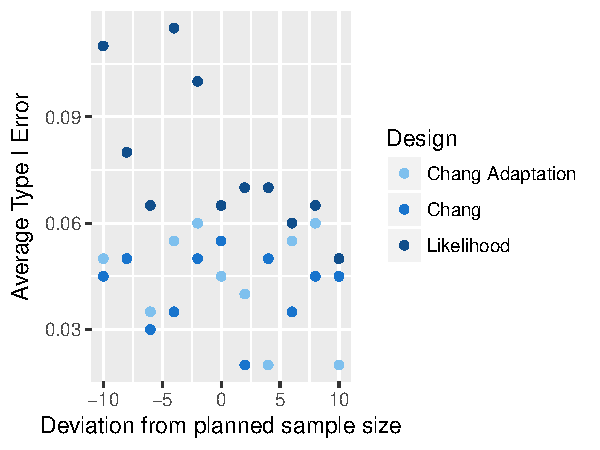
\includegraphics{plot1-1} }

\end{Schunk}
\end{figure}
\end{landscape}


\begin{landscape}
\begin{figure}[]
\caption{Monte Carlo Simulation of Average Type I Error Rates and Power of 20 Simon-like Designs when Stage I Sample Size Deviates from Planned for Attained Designs ($n_t^{\ast\ast} = n_t$) Number of Simulations = 10000.}
\begin{Schunk}


\centerline{\includegraphics{plot2-1} }

\end{Schunk}
\end{figure}
\end{landscape}

\begin{figure}[]
\caption{Monte Carlo Simulation of the Average of the Average Type I and Type II Error Rates of 20 Simon-like Designs when Stage I Sample Size Deviates from Planned for Attained Designs ($n_t^{\ast\ast} = n_t$) Number of Simulations = 10000.}
\begin{Schunk}


\centerline{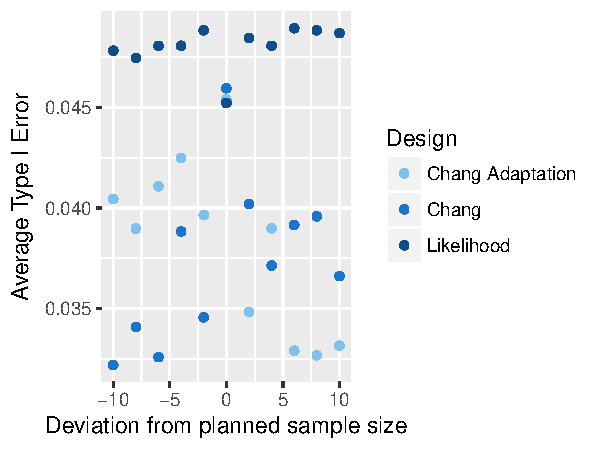
\includegraphics{unnamed-chunk-12-1} }

\end{Schunk}
\end{figure}

%%%%%%%%%%%%%%%%%%%%%%%%%%%%%%%%%%%%%%%%%%%%%%%%%%%%%%%%%%%%%%
%----------------Discussion--------------------------------%
\newpage
\chapter{Discussion and Conclusion}

%%%%%%%%%%%%%%%%%%%%%%%%%%%%%%%%%%%%%%%%%%%%%%%%%%%%%%%%%%%%%%
Deviations from the planned second stage sample size has been better studied than deviations from the planned first stage sample size. Some methods have been proposed on decision rules, and Koyama and Chen had introduced a redesign when the first stage sample size is as planned. Because the calculation of a proper p-value in this case is more straightforward than when stage I differs, there may be less literature proposing these redesigns. Though, one could calculate a p-value ignoring the sample paths for deviations in either the first or second stage as if the two-stage design were a single stage with attained values. If this were done, the decision could be different than that of the proper p-value which considers sample paths, and how to decide how small the p-value is needed in order to determine statistical significance is unclear.\\
\indent We focused our investigation and results on deviations from the planned first stage sample size. One argument against redesigning these trials in the first place could be that researchers always have the option to simply wait until stage I sample size is met. In practice, though, some ethical matters may arise that would give the researcher incentive to evaluate the first stage prematurely. For instance, if a new regimen appears to be more beneficial than historical treatments, but statistical requirements prevent new subjects from being enrolled until all currently enrolled subjects record responses, a researcher may consider this unethical. In this case, $n_1^{\ast\ast} < n_1$ where $n_1^{\ast\ast}$ would be subjects who have recorded responses. Having a decision rule for a case such as this would alleviate some discomfort from both the researcher and statistician, though abuse of new decision rules would be discouraged. \\
\indent We suggest a redesign of a trial for attained sample sizes using the planned total sample size for practical reasons such as resources and inability to stray far from the planned design. A numerical study also suggested that it may be desirable to redesign trials using the planned total sample size because it better controls type I error for all attained methods and power is closer to the nominal power more often. Furthermore, if one employs Chang \textit{et al.}'s method, the sample size is radical in the first stage, and the resulting probability of continuing is less than 0.05, it will be impossible for a type I error to occur. This will then reduce the two-stage design to a one-stage design which is considerably different than the planned design, so this is further support for using the planned total sample size.  Assuming that redesigns use the planned total sample size, results from different two-stage designs were presented.  Chang \textit{et al.} and the Olson and Koyama methods primarily differ when there are extreme sample size shifts. This is most likely due to the nature of their methods and their primary goals of maintaining type II error spending versus probability of early termination. \\
\indent Recommending the use of these designs in practice will depend on the desire of statistical approach of the researcher. Blume states, "Hypothesis testing procedures do not place any interpretation on the numerical value of the likelihood ratio. The extremeness of an observation is measured, not by the magnitude of the likelihood ratio, but by the probability of observing a likelihood ratio that large or larger. It is the tail area, not the likelihood ratio, that is the meaningful quantity in hypothesis testing" \cite{Blume2002}. Thus, the primary argument for using Chang \textit{et al.}'s or the OK method is in the case that the researcher does not want to abandon hypothesis testing.  If the researcher prefers to use a traditional frequentist approach with hypothesis testing, it may be recommended that the Olson and Koyama's approach is used because it results in higher average power across deviations. Because it may be of concern that researchers take advantage of the ability to deviate from the planned design, Olson and Koyama's method also penalizes deviation by resulting in a higher probability of early termination when there is under-accrual than Chang \textit{et al}'s method. \\
\indent Overall, there are many advantages to using a Likelihood two-stage design. One advantage to the Likelihood design is that it is able to add cohorts of subjects at the end of the second stage if weak evidence is obtained without threatening frequentist properties such as type I error. Another advantage to the Likelihood approach is that inference is more straightforward because one is not concerned with error rates or p-values. The likelihood is unaffected by the number of looks at the data and the evidence is independent of the probability of observing misleading evidence \cite{Blume2002}. Though we don't consider calculating p-values when stage I differs from planned, it would be complicated if one wished to do so, whereas Likelihood methods would not require this because evidence is represented by a simple calculation of the likelihood ratio.  Likelihood designs are also more generalizable. The Likelihood two-stage approach could be generalized easily to three stages, whereas the Chang \textit{et al.} and OK designs would not be able to generalize in such a way. In this paper, though, we are very much restricting the Likelihood design and not taking full advantage of its natural characteristics. One could simply use a pure Likelihood design and avoid traditional frequentist issues altogether. \\
\indent In general, though, if a researcher wanted to design a study using the restricted designs as described in this paper, the OK design and the Likelihood design are highly competitive and achieve similar results when the probability of early termination is reasonable (i.e. above 50\%). One design may be more favorable than the other depending on the hypotheses being tested and the amount of over- or under-enrollment. \\
\indent We do not consider redesigns when both the first and second stage accrual are not as planned because if one is interested in prespecifying stopping criteria for sample size deviations, the number of combinations needed to be specified in order to prespecify the exact combination that will occur is unreasonable. Though, these attained designs are able to accommodate if this is desired. Lastly, a primary concern that we have with redesigning trials for unplanned sample sizes is that researchers could take advantage of the these new stopping criteria and stray from the planned design too often. It is for this reason that one may consider adapting Chang \textit{et al.}'s design using a very conservative rule in the first stage and have the probability of early termination under the null always be higher than planned. When deviations are extreme, especially where there is underacrrual, evaluating the trial early would be highly penalized by potentially having a very high probability of early termination. Overall, intentional early or late evaluation of the first stage without sound reason is highly discouraged and will not result in optimal statistical properties. 




%%%%%%%%%%%%%%%%%%%%%%%%%%%%%%%%%%%%%%%%%%%%%%%%%%%%%%%%%%%%%%
%------------------------------------------------%
%%%%%%%%%%%%%%%%%%%%%%%%%%%%%%%%%%%%%%%%%%%%%%%%%%%%%%%%%%%%%%

%%%%%%%%%%%%%%%%%%%%%%%%%%%%%%%%%%%%%%%%%%%%%%%%%%%%%%%%%%%%%%
%-------------- BIBLIOGRAPHY--------------------------------------%
%%%%%%%%%%%%%%%%%%%%%%%%%%%%%%%%%%%%%%%%%%%%%%%%%%%%%%%%%%%%%%


%\bibliographystyle{apacite}
\bibliographystyle{ieeetr}
\bibliography{/Users/mollyolson/Documents/Vanderbilt/Masters_Thesis/ThesisRepo/thesisBib}		

\end{document} 


